%%% & --translate-file=cp1250pl
%% ************ AKADEMIA GÓRNICZO-HUTNICZA W KRAKOWIE **************
%% ***************** Wydział Matematyki Stosowanej ***************** 
%% ****************** PRACA MAGISTERSKA w LaTeX-u ******************
%%    autor: Tomasz Czyż
%%    Copyright (C) 2003 by ------
%% ************************* Plik główny *************************

%%
%% ======== PREAMBUŁA ======== 
%%
\documentclass[oik, pdftex, robocza, man]{mgrwms}

\usepackage[utf8]{inputenc}  % opcja latin2 dla Linux
\usepackage{amsmath}           % łatwiejszy skład matematyki
\newcommand\numberthis{\addtocounter{equation}{1}\tag{\theequation}}
\DeclareMathOperator*{\esssup}{ess\,sup}
\DeclareMathOperator*{\argmax}{arg\,max}
\DeclareMathOperator*{\argmin}{arg\,min}
\DeclareMathOperator*{\conv}{conv}
\usepackage{amssymb}
\usepackage{bbm}
\usepackage{latexsym}
\usepackage{amsthm}
\usepackage{enumerate}
\usepackage{enumitem}
\usepackage{mathtools}
\usepackage{color}
\usepackage{float}
\usepackage{graphicx}
\graphicspath{ {./images/} }

\usepackage[polish]{babel}
\usepackage[OT4]{fontenc}
\usepackage{polski}

\allowdisplaybreaks
%% <<<< BiBTeX >>>>
% \bibliographystyle{ddabbrv}
% \nocite{*}


\begin{document}
%%
%% ======== METRYCZKA PRACY ========
%%
\title{ \LARGE Aproksymacja funkcji kawałkami regularnych przy użyciu informacji dokładnej i niedokładnej}
\author{Tomasz Czyż}
\promotor{dr Maciej Goćwin}
\nralbumu{290565}
\maketitle

\slowakluczowe{słowa kluczowe}
\keywords{keywords}
%%
%% ======== MAKRA ========
%%
%-> Miejsce na nasze makra (jedno z wielu ;). Lepszym pomysłem będzie jednak 
%-> umieszczenie ich w osobnym pliku i wczytanie poleceniem \input
%%
\newtheorem{thm}{Twierdzenie}[chapter]
\newtheorem{lemma}[thm]{Lemat}
\newtheorem{stw}[thm]{Stwierdzenie}
\newtheorem{cor}[thm]{Wniosek}
\newtheorem{obs}[thm]{Obserwacja}
\newtheorem{uw}[thm]{Uwaga}
\newtheorem{df}[thm]{Definicja}
\newcommand{\E}{\mathbb{E}}
\newcommand{\R}{\mathbb{R}}
\newcommand{\Pra}{\mathbb{Pra}}
\newcommand{\F}{\mathcal{F}}
\newcommand{\1}{\mathbbm{1}}
\newcommand{\Galphabeta}{\mathcal{G}_{r,\varrho}([\alpha,\beta])}
\newcommand{\G}{\mathcal{G}_{r,\varrho}}
\newcommand{\wor}{\mathrm{wor}}
\newcommand{\reg}{\mathrm{reg}}
\newcommand{\cost}{\mathrm{cost}}
\newcommand{\comp}{\mathrm{comp}}
\newcommand{\po}{\hat{t}}

\makeatletter
\newcommand*{\defeq}{\mathrel{\rlap{%
                     \raisebox{0.3ex}{$\m@th\cdot$}}%
                     \raisebox{-0.3ex}{$\m@th\cdot$}}%
                     =}
\let\c@table\c@figure
\makeatother

%%
%% ======== SPIS TREŚCI ========
%%

\tableofcontents

%%
%% ======== STRESZCZENIE PRACY (POLSKIE) ========
%%

\begin{streszczenie}
    Streszczenie
\end{streszczenie}

%%
%% ======== STRESZCZENIE PRACY (ANGIELSKIE) ========
%%

\begin{abstract}
    Abstract
\end{abstract}

%%
%%
%% ======== GŁÓWNA CZĘŚĆ PRACY ========
%%
%%

%%
%% ==== WSTĘP ====
%%

\begin{wstep}[Wprowadzenie]
    Aproksymacja funkcji oparta na dostępnej inforamcji jest problemem badanym od lat. Powstają coraz bardziej zaawansowane algorytmy, działające przy coraz słabszych założeniach o funkcji. Często jednak w rozważaniach teoretycznych pomijany jest czynnik zewnętrzny, który może powodować zaburzenia dostępych informacji. W tej pracy rozważamy, jaki wpływ na wyniki numeryczne może mieć zaniedbanie tego faktu.

    W rozważaniach zakładamy, że mamy dostęp tylko do częściowej informacji o funkcji, a jedynym źródłem informacji jest tzw. \textit{wyrocznia}. To podejście ma praktyczne uzasadnienie w obliczeniach numerycznych, gdzie odwołania do wyroczni odpowiadają ewaluacjom funkcji. Na ogół wartości, które otrzymujemy są wynikiami pewnych pomiarów (np. fizycznych), które zawsze są obarczone pewnym błędem. Uwzględnienie zaburzenia danych jest więc intuicyjne.
    
    Dodatkowo, najczęściej spotykane dane cechują się pewnym stopniem nieregularności. Z tego powodu powstaje wiele prac, w których przyjmuje się słabsze założenia na aproksymowaną funkcje. W tej pracy rozważać będziemy funkcje, które zawierają dokłanie jeden, nieznany punkt osobliwy, w którym nie musi być zachowna ciągłości czy różniczkowalność.

    Mówimy, że funkcja skalarna $g$ jest $(r, \varrho)$-regularna na przedziale $[a,b]$, jeśli $g \in C^{r}([a,b])$ oraz $g^{(r)}$ jest Hölderowsko ciągła z wykładnikiem $\varrho \in (0,1]$. Rozważmy przestrzeń $F_{r,\varrho}$ $T$-okresowych funkcji $f$, które składają się z dwóch $(r,\varrho)$-regularnych części oddzielonych nieznanym punktem osobliwym $\po_{f}$. Założenie o okresowości funkcji zostało wprowadzone, aby uprościć prezentację problemu. Po kilku techniczych modyfikacjach wszystkich wyniki działają dla funkcji nieokresowych.

    W celu porównania wpływu zaburzenia informacji przedstawimy dwa algorytmy z artukułów \cite{AoP} i \cite{CoDF}. Pierwszy z nich bazuje na wielomianach Lagrnage'a i jego analiza nie uwzględnia zaburzenia danych wejściowych. Algorytm z \cite{AoP} dopuszcza informacje niedokładną, a kluczowy krok opiera się na różnicach dzielonych. 

    Oba algorytmy stosują podejście adaptacyjne do wybierania dodatkowych ewaluacji funkcji, to znaczy, wybór kolejnych punktów jest uzależniony od wcześniejszych wartości. Skuteczność algorytów adaptacyjnych i nieadaptacyjnych została szeroko przeanalizowana dla wielu klas funkcji przy założeniu, że informacja jest dokładna. Użycie adaptacji w obu z omawianych algorytmów jest uzasadnione wynikami z m.in. \cite{PoA}. W artukule pokazano, że błąd $L_{p}$-aprkosymacji funkcji z jednym punktem osobliwym dla algorytmów nieadaptacyjnych używających $n$ ewaluacji funkcji nie może być lepszy niż $n^{1/p}$, przy czym algorytmy adaptacyjne osiągają optymalne tępo zbieżności $n^{-r}$.

    W tej samej pracy udowodniono również, że dla funkcji posiadających wiele punktów osobliwych tępo zbieżności błądu najgorszego przypadku względem normy $L_{p}$ maleje do $n^{1/p}$. Z tego powodu skupiamy się na funkcjach z jedną osobliwością. Wyniki te przytoczymy w rozdziale \ref{rozdzial:ograniczenia_na_blad}.

    W rozdziale \ref{rozdzial:algorytmy} przedstawimy algorytmy z prac \cite{AoP} i \cite{CoDF}.

\end{wstep}


\chapter{Definicje}


\section{Informacja, algorytm, aproksymacja}


    W tym rozdziale wyjaśnijmy co rozumiemy przez aproksymację i w jaki sposób ją otrzymujemy. W tym celu wprowadzimy fundamentalne pojęcia, takie jak operator rozwiązania, informacja niedokładna oraz algorytm. Szczególną uwagę poświęcimy informacji która, mówiąc w skrócie, jest tym co wiemy o problemie do rozwiązania. Głównym założeniem tej pracy jest warunek, że informację o funkcji otrzymujemy z pewnym błędem. Taką informację nazywamy \textit{niedokładną} lub \textit{zaburzoną}.

    Niech $F$ będzie przestrznią liniową a $G$ przestrzenią unormowaną, obie nad ciałem liczb rzeczywistych. Odwzorowanie 
    \begin{equation*}
        S : F \rightarrow G
    \end{equation*}
    nazywamy \textit{operatorem rozwiązania}. Elementy z $f$ z $F$ nazywane są \textit{problemami}, a elementy $S(f)$ \textit{rozwiązaniami}. Dla każdego problemu $f$ chcemy obliczyć aproksymację rozwiązania $S(f)$. Niech $U(f)$ będzie obliczoną aproksymacją.

    Niech $\varepsilon \geq 0$. Mówimy, że $U(f)$ jest $\varepsilon$-aprkosymacją funkcji $f$ wtedy i tylko wtedy, gdy $\| S(f) -  U(f)\| \leq \varepsilon$. Celem jest znalezienie takiej aproksymacji $U(f)$, że jest ona $\varepsilon$-aprkosymacją dla wszysktich elementów $f$ z $F$. Aby to zrobić potrzebujemy posiadać pewną wiedzę o $f$.

    \textit{Operatorem informacji (lub informacją)} nazywamy odwzorowanie
    \begin{equation*}
        N : F \rightarrow 2^{Y},
    \end{equation*}
    gdzie Y jest zbiorem skończonych ciągów liczb rzeczywistych, $ Y \subset \bigcup^{\infty}_{n=1} \R^{n}$, czyli $N(f)$ jest pozbiorem $Y$.
    Na ogół nie mamy dostępu do pełnej wiedzy o funkcji, dlatego musimy założyć, że możemy zbierać informacje o $f$ poprzez pewnien funkcjonał $L(f)$, gdzie $L : F \rightarrow \R$.
    
    Przez $\Lambda$ oznaczmy klasę dopuszczalnch operacji $L$, czyli $L \in \Lambda$ wtedy i tylko wtedy, gdy $L(f)$ może zostać obliczone dla każdego elementu $f$ z $F$. Rozważmy teraz dwa sposoby doboru inforamcji. Inforamcję $N$ nazywamy nieadaptacyjną wtedy i tylko wtedy, gdy istnieje $L_{1}, \ldots, L_{n} \in \Lambda$ takie, że
    \begin{equation*}
        N(f) = \left[ L_{1}(f), L_{2}(f), \ldots, L_{n}(f) \right] \; \forall f \in F.
    \end{equation*}
    W tym przypadku poszczególne funkcjonały informacji zależą tylko od elementu $f$ i są obliczane niezależnie.
    Ogólniejszą klasą jest informacja adaptacyjna, w której możemy wybierać wartości funkcjonałów bazując na poprzednich wynikach. Mówiąc dokładniej, informacja $N$ jest adaptacyjna wtedy i tylko wtedy, gdy
    \begin{equation*}
        N(f) = \left[ L_{1}(f), L_{2}(f; y_{1}), \ldots, L_{i}(f; y_{1}, \ldots, y_{n(f)-1}) \right],
    \end{equation*}
    gdzie $y_{1} = L(f_{1})$ i $y_{i} = L_{i}(f; y_{1}, y_{2}, \ldots, y_{i-1})$ dla $i=2,3,\ldots,n(f)$. Musimy również założyć, że $L_{i}(\cdot;y_{1}, \ldots, y_{i-1})$ należą do operacji dozwolonych. W przypadku informacji adaptacyjnej nie możemy z góry określić liczby operacji na problemie $f$, ponieważ jest to dynamicznie ustalne podczas procesu oblicznia kolejnych wartości $y_{i}$.

    Warto zauważyć, że jeśli rozważany problem wymaga obliczenia bardzo dużej ilości informacji o funkcji w krótkim czasie, to zastosowanie informacji nieadaptacyjnej może przyśpieszyć proces, ze względu na możliwość zrównoleglenia obliczeń. W przypadku adaptacyjnym kolejność obliczeń ma znaczenie, więc informacje musimy pozyskiwać sekwencyjnie, co zazwyczaj jest wolniejsze.

    W niniejszej pracy zakładamy, że $f$ jest funkcją, a jedynymi dostępnymi funkcjonałami informacji są wartości funkcji w punktach. Informację nieadaptacyjną oraz adaptacyjną możemy więc zapisać w postaci $N(f) = \left[ f(t_{1}), f(t_{2}), \ldots, f(t_{n(f)}) \right]$. Jeżeli $n(f) = n$ i punkty $t_{i}$ otrzymujemy \textit{a priori}, wtedy $N$ jest nieadaptacyjna. Natomiast, jeżeli $n(f)$ różni się lub wybór punktów $t_{i}$ jest zależny od $f(t_{1}), f(t_{2}), \ldots, f(t_{i-1})$, to $N$ jest adaptacyjna.

    Kluczowym założeniem jest fakt, że informacje o funkcji uzyskujemy z pewnym błędem. Mówiąc dokładniej, inforamacje o funkcji przyjmują postać $y_{i} = f(x_{i}) + e_{i}$, dla $1 \leq i \leq n$, gdzie $|e_{i}| \leq \delta$ to tak zwany \textit{szum}.
    
    Dla przykładu, dla informacji nieadaptacyjnej składającej się z zaburzonych ewaluacji funkcji $f$ w punktach $t_{1}, \dots, t_{n}$ z precyzją $\delta$, mamy
    \begin{equation*}
        N(f) = \{y \in \R^{n} : \quad |y_{i} - f(t_{i})| \leq \delta, \quad 1 \leq i \leq n\}.
    \end{equation*}
    
    Każdy element $y \in N(f)$ będziemy nazywać \textit{informacją o $f$}. Zauważmy, że dla $\delta = 0$, zbiór $N(f)$ ma dokładnie jeden element dla wszystkich $f \in F$, tzn. informacja $N$ jest \textit{dokładna}. Zakładamy, że $N(f)$ jest niepuste dla wszystkich $f \in F$. W przypadku, gdy istnieje $f$ dla którego $N(f)$ ma przynajmniej dwa elementy, wtedy informacja jest \textit{niedokładna}.

    Znając informację $N(f)$ możemy obliczyć aproksymację $f$ używając \textit{algorytmu} $\varphi$, w postaci odwzorowania
    \begin{equation*}
        \varphi : Y \rightarrow G.
    \end{equation*}
    Dostajemy, że aproksymacja $U(f) = \varphi(N(f))$, czyli algorytm $\varphi$ używa informacji $N(f)$, aby wyprodukować element z $G$, który aproksymuje $S(f)$.

    W tej pracy rozważamy zagadnienie aproksymacji pewnych funkcji skalarnych, używając skończonej liczby wartości funkcji, przy założeniu, że błąd aproksymacji jest mierzony w normie $L^{p}$ ($1 \leq p \leq \infty$). A zatem operator rozwiązania $S$ jest odwzorowaniem identycznościowym prowadzącym z przestrzeni funkcji $F$ w przestrzeń $L^{p}$, natomiast błąd aproksymacji $f \in F$ otrzymanej algorytmem $\varphi : Y \rightarrow L^{p}(0,T)$ z użyciem inforamcji $y \in N(f)$ wynosi
    \begin{equation*}
        \|f-\varphi(y)\|_{L^p} = \left( \int_{0}^{T} |(f-\varphi(y))(x)|^p \,dx  \right)^{1/p} \quad \text{ dla } \; 1 \leq p < \infty
    \end{equation*}
    oraz
    \begin{equation*}
        \|f-\varphi(y)\|_{L^\infty} = \esssup_{0 < x \leq T} | (f - \varphi(y))(x) |.
    \end{equation*}


    Dla przykładu, niech F będzie przestrzenią ciągłych funkcji rzeczywistych dwukrotnie różniczkowalnych $f: [0,1] \rightarrow \R$, a $G=L_{2}(0,1)$. To oznacza, że $S(f) = f$, a dla $t_{i} \in [0,1]$ opartor informacji dany jest przez
    \begin{equation*}
        N(f)=\left\{y \in \R^{n} \mid \sum_{i=1}^{n}\left(y_{i}-f\left(t_{i}\right)\right)^{2} \leq \delta^{2}\right\},
    \end{equation*}
    gdzie $y$ odpowiada $n$ obserwacjom $f(t_{i})$ dla $1 \leq i \leq n$, z precyzją $\delta$ każda. Przykładem algorytmu aproksymujęcego funkcję $f$ może być konstrukcja funkcji sklejanej $l: [0,1] \rightarrow \R$, czyli takiej funkcji, że $l$ jest wielomianem na każdym podprzedziale $(t_{i}, t_{i+1})$ podziału $t_{1} < \ldots < t_{n}$.


    % Naszym zadaniem jest aproksymacja elementów $S(f)$ dla $f$ należącego do $E \subset F$, bazując wyłącznie na informacji zaburzonej o $f$.


\section{Model obliczeniowy}


    W ogólności, optymalność algorytmu oraz złożoność problemu zależą od przyjętego modelu obliczeniowego. Model jest określony poprzez sposób w jaki błąd i koszt algorytmu są zdefiniowane. 
    
    Jeżeli za błąd i koszt przyjmujemy wydajność na najtrudniejszym spośród wszystkich problemów w danej klasie, wtedy mówimy o \textit{modelu najgorszego przypadku}. Innymi często rozważanymi modelami są: model probablistyczny, średni, mieszany, losowy czy asymptotyczny, jednak nimi nie będziemy zajmować się w tej pracy.

    Niech $N : F \rightarrow 2^{Y}$ będzie operatorem inforamcji a $S: F \rightarrow G$ operatorem rozwiązania dla $G=L^{p}$. Poprzez \textit{błąd najgorszego przypadku} algorytmu $\varphi : Y \rightarrow L^{p}$ na zbiorze $E \subset F$ rozumiemy:
    \begin{equation*}
        e_{p}^{\wor}(\varphi, N, E) = \sup_{f \in E} \sup_{y \in N(f)} \|S(f) - \varphi(y) \|_{L^{p}}
    \end{equation*}

    Celem jest znalezienia algorytmu, który minimalizuje błąd najgorszego przypadku względem wszystkich algorytmów w danej klasie. Algortym osiągający to minimum nazywamy \textit{optymalnym}.

    W tej pracy rozważamy algorytmy aprosymujące funkcje z osobliwością, które wykorzystują określoną liczbę wartości funkcji. Oznaczmy przez $\mathcal{N}(n, \delta)$ klasę wszystkich (adaptacyjnych) informacji $N$, które używają co najwyżej $n$ ewaluacji funkcji, z precyzją $\delta$ każda. Wtedy przez \textit{minimalany błąd najgorszego przypadku} w klasie $E$, który może zostać osiągnięty przez algorytm używający informacji o co najwyżej $n$ wartościach funkcji z precyzją $\delta$ rozumiemy:

    \begin{equation*}
        r^{\wor}_{p}(n, \delta, E) = \inf\{ e_{p}^{\wor}(\varphi, N, E) : \; \varphi \text{ używa } N \in \mathcal{N}(n, \delta) \}
    \end{equation*}


    W tej pracy porównujemy dwa algorytmy aproksymujęce funkcje z osobliwością, które osiągają błąd na takim samym, optymalnym, poziomie błędu najgorszego przypadku, jednak tylko w przypadku jednego z nich w analizie zostało uwzględione zaburzenie informacji.

    Drugą cechą modelu obliczeniowego jest koszt algorytmu. Może się na niego składać zarówno koszt uzyskania informacji o wartości funkcji, jak i koszt operacji arytmetycznych potrzebnych do obliczenia algorytmu. Ponieważ zakładamy, że ewaluacje wartości funkcji obarczone są pewnym błędem, który może znacząco przewyższać błędy wynikające z operacji arytmetycznych, przyjmujemy, że koszt algorytmu $\varphi$ jest równy tylko kosztowi uzyskania informacji o wartości funkcji $f$, czyli
    \begin{equation*}
        \cost(\varphi, f) = n,
    \end{equation*}
    Koszt algorytmu w całej klasie $F$ ma postać
    \begin{equation*}
        \cost(\varphi, F) = \sup_{f \in F} \cost(\varphi, f)
    \end{equation*}
    Niech $\varepsilon > 0$. $\varepsilon$-złożoność najgorszego przypadku klasy $F$ mierzymy w następujący sposób
    \begin{equation*}
        \comp(\varepsilon, F) = \inf \{\cost(\varphi, F), | \text{ $\varphi$ - algorytm oraz } \sup_{f \in F} \sup_{t \in [a,b]} \|f(t) - \varphi(t)\| \leq \varepsilon\}.
    \end{equation*}
    Celem jest otrzymanie ścisłych granic na $\comp(\varphi, F)$, gdy $\varepsilon \rightarrow 0$.

    Do określania błędu będziemy używać notacji $\varOmega$, $\varTheta$, $\mathcal{O}$, $\textit{o}$ (wersji Knutha). Gdy dwie funkcje $f$ i $g$ zdefiniowane na $\R_{+}$ i przyjmują wartości nieujemne, to piszemy $f(x) = \varOmega\left( g(x) \right)$ wtedy, gdy istnieją dodatnie stałe $c_{1}$ i $c_{2}$, takie że $f(x) \geq c_{1} g(x)$ dla $x \in [0, c_{2}]$. Przez $f(x) = \varTheta\left( g(x) \right)$ rozumiemy $f(x) = \varOmega\left( g(x) \right)$ and $g(x) = \varOmega\left( f(x) \right)$, czyli istnieją takie stałe $c_{1}$, $c_{2}$ i $c_{3}$, że $c_{1} g(x) \leq f(x) \leq c_{2} g(x)$ dla $x \in [0, c_{3}]$. Natomiast przez $f(x) = \mathcal{O}(g(x))$ rozumiemy, że $g(x) = \varOmega(f(x))$, a przez $f(x) = \textit{o}(g(x))$ rozumiemy, że $\displaystyle \lim_{x \rightarrow 0} \frac{f(x)}{g(x)} = 0$.



\section{Klasy funkcji} \label{rozdzial:klasy_funkcji}

    Wprowadzimy teraz dwie definicje klasy funkcji kawałkami regularnych użyte w artykułach \cite{CoDF} i \cite{AoP}. 

    Przez funkcje $r$-regularne rozumiemy funkcje, których pochodne do rzędu $r$ istnieją w całej dziedzinie oraz są one ciągłe. \\
    Dla liczby całkowitej $ r \geq 0$, $\varrho \in (0,1]$ oraz $a < b$, przez $H_{r, \varrho}(a,b)$ oznaczamy klasę funkcji $g: [a,b] \rightarrow \R$ takich, że $g \in C^r([a, b])$ i $g^{(r)}$ jest Hölderowsko ciągła z wykładnikiem $\varrho$, tzn.
    \begin{equation*}
        c(g) := \sup_{a \leq x \leq y \leq b} \frac{|g^{(r)}(x) - g^{(r)}(y)|}{|x-y|^{\varrho}} < \infty.
    \end{equation*}
    Dla danego $T > 0$ niech $F_{r, \varrho} = F_{r, \varrho}(T)$ będzie przestrzenią funkcji $f: \R \rightarrow \R$ spełniających następujące warunki: istnieje $\po_{f} \in [0, T)$ i $g_f \in H_{r, \varrho}(0,T)$ takie, że
    \begin{equation*}
        f(lT + \po_f + x) = g_f(x) \quad \text{dla każdego} \quad l = 0, \pm 1, \pm 2, \ldots \quad \text{i} \quad x \in [0, T)
    \end{equation*}
    Można powiedzieć, że $f$ jest 'kopią' $g_f$ na każdym z przedziałów $(lT + \po_f, (l + 1)T + \po_f]$ i $f$ jest prawostronnie ciągła w $lT + \po_f$. W związku z tym wszystkie punkty, które różnią się między sobą o wielokrotność $T$ będą uważane za identyczne. Dla przykładu, jeżeli $0 < x_1 \leq T < x_2 \leq 2T$, to przedział $(x_1, x_2]$ będzie utożsamiany z $(x_1,T] \cup (0, x_2 - T] \subset (0, T]$.

    \begin{figure}[h!]
        % \centering
        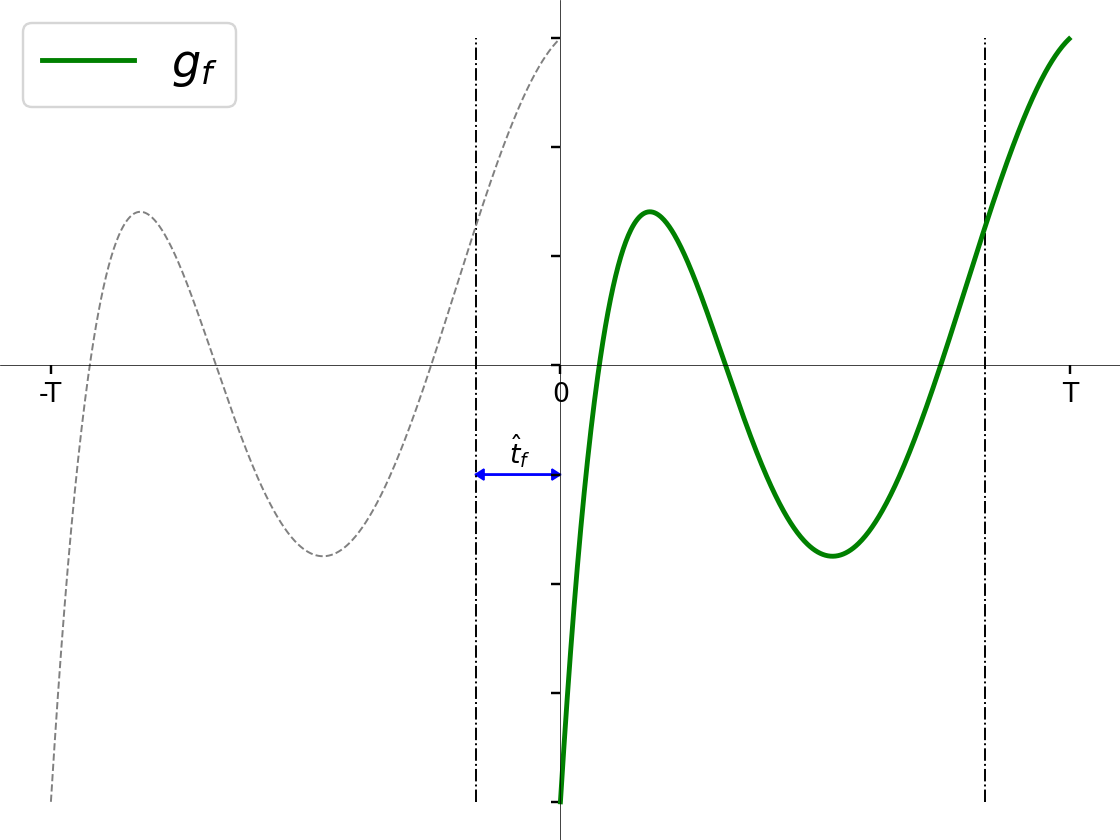
\includegraphics[width=.45\linewidth]{g_f_plot.png}
        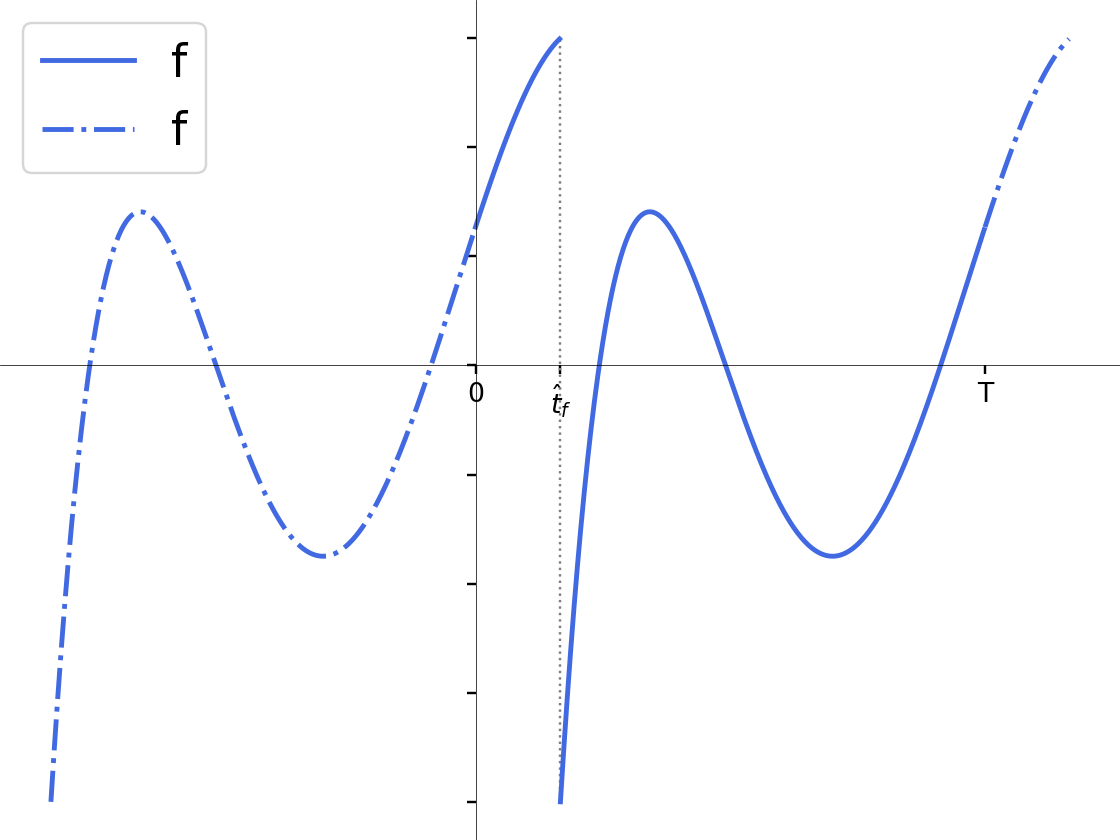
\includegraphics[width=.45\linewidth]{f_plot.png}
    \end{figure}


    Przez $\Delta_f^{(j)}$ ozanaczmy \emph{skoki nieciągłości} dla kolejnych pochodnych $f$ w punkcie nieciągłości $\po_f$,
    \begin{equation*}
        \Delta_f^{(j)} = f^{(j)}(\po_f^+) - f^{(j)}(\po_f^-) = g_f^{(j)}(0) - g_f^{(j)}(T) \quad 0 \leq j \leq r,
    \end{equation*}

    Ze względu na zachowanie się funkcji w punkcie osobliwym, rozróżniamy następujące klasy funkcji
    \begin{equation*}
        \begin{split}
            \mathcal{K} & = \{f = c \1_{\R}, c \in \R \}, \\
            \mathcal{H}_{r, \varrho} & = \{ f \in F_{r, \varrho}: c(g_{f}) \leq 1, \Delta_{f}^{(j)} = 0 \text{ dla każdego } 0 \leq j \leq r\} \\
            \mathcal{F}_{r, \varrho}^{C} & = \{ f \in F_{r, \varrho}: c(g_{f}) \leq 1, \Delta_{f}^{(0)} = 0 \} \\
            \mathcal{F}_{r, \varrho}^{D} & = \{ f \in F_{r, \varrho}: c(g_{f}) \leq 1, | \Delta_{f}^{(0)} | \leq 1 \} \\
            \mathcal{F}_{r, \varrho} & = \{ f \in F_{r, \varrho}: c(g_{f}) \leq 1 \}. \\
        \end{split}
    \end{equation*}
    Oczywiście
    \begin{equation*}
        \mathcal{K} \subset \mathcal{H}_{r, \varrho} \subset \mathcal{F}_{r, \varrho}^{C} \subset \mathcal{F}_{r, \varrho}^{D} \subset \mathcal{F}_{r, \varrho}.
    \end{equation*}


    Algorytm przedstawiony w  \cite{CoDF}, oryginalnie bazuje na lekko zmodyfikowanych klasach funkcji, co wynika z innej natury problemu rozważanego w pracy. Dla spójności i lepszego przedstawiania problemu wprowadzimy oryginalnie rozważane klasy funkcji i sprecyzujemy różnice między klasami przedstawionymi wcześniej.

    Niech $L_{0}, L_{r}, D_{0}, D_{1}, \ldots, D_{r}$ będą dodatnimi stałymi. Wprowadźmy klasę funkcji regularnych
    \begin{equation*}
        \begin{aligned}
        G_{r, \varrho}^{\reg}([a, b])= &\left\{g:[a, b] \rightarrow \R^{d} \mid g \in C^{(r)}([a, b]),\left\|g^{(j)}(x)\right\| \leq D_{j}, j=0,1, \ldots, r\right. \\
                                      &\left.\left\|g^{(r)}(x)-g^{(r)}(y)\right\| \leq L_{r}|x-y|^{\varrho},\|g(y)-g(x)\| \leq L_{0}|y-x|, x,y \in [a, b]\right\}.
        \end{aligned}
    \end{equation*}

    Rozważmy następującą klasę $\G([a, b])$ funkcji $g:[a, b] \rightarrow \R^{d}$ z co najwyżej jednym (nieznanym) punktem osobliwym $\hat{t}_{g}$. Funkcja $g:[a, b] \rightarrow \R^{d}, g=\left[g^{1}, g^{2}, \ldots, g^{d}\right]^{T}$, należy do $\G([a, b])$, jeśli istnieje punkt $\po_{g} \in (a, b)$ taki, że 
    \begin{equation*}
        g \in G_{r, \varrho}^{\reg}\left(\left[a, \po_{g}\right)\right) \cap G_{r, \varrho}^{\reg}\left(\left[\po_{g}, b\right]\right)    
    \end{equation*}
    oraz lewostronna granica każdej składowej pochdnej $\left(g^{k}\right)^{(j)}$ istnieje w $\hat{t}_{g}$. W punkcie osobliwym $\hat{t}_{g}$, pochodne są rozumiane jako prawostronne.
    
    Dla funkcji $g \in \G([a,b])$ definiujemy wielomian
    \begin{equation} \label{eq:26}
        s_{g}(t)=\sum_{j=0}^{r} \frac{1}{j !} \Delta_{g}^{(j)}\left(t-\po_{g}\right)^{j}, \quad t \in [a, b],
    \end{equation}
    gdzie $\Delta_{g}^{(j)}$ jest wektorem skoków w punkcie osobliwym zdefiniowanym jak wcześniej.
    Zauważmy, że $g \in \G$ wtedy i tylko wtedy, gdy
    \begin{equation} \label{eq:32:druga_def_G_r_rho}
        g(t) = h(t) + \1_{[\po, b]}(t) \cdot s_{g}(t), \quad t \in [a, b],
    \end{equation}
    gdzie $h \in G^{\reg}_{r, \varrho}$.

    Jeżeli $\Delta_{g}^{(j)}=0$ dla wszystkich $j=0,1, \ldots, r$, wtedy $g$ jest regularna, czyli $g \in G_{r, \varrho}^{\reg}([a, b])$. Jeżeli $g \in \G([a, b])$ i $\Delta_{g}^{(0)}=0$, wtedy $g$ jest Lipschitzowsko ciągła w $[a, b]$.

    Definicja klasy $G_{r, \varrho}^{\reg}$ różni się od definicji  $F_{r, \varrho}$ dopuszczeniem wielowymiarowości funkcji $g$, bardziej ogólnym podejściem do parametrów klasy oraz brakiem założenia o okresowości. Przyjęcie, że funkcje prowadzą w $\R$ ułatwia rozważania praktyczne, a wyniki teoretyczne można łatwo uogólnić. W przypadku drugiej różnicy, ponieważ w tej pracy skupiamy się na wynikach numerycznych, przyjęcie za jedyny parametr klasy $c(g_{f}) = 1$ jest uzasadnionym uproszczeniem. Funkcję zawsze możemy przemnożyć przez stałą, aby otrzymać odpowiedni parameter. Natomiast założenie dotyczące okresowości ma jedynie na celu uprościć analizę algorytmu i może zostać łatwo uogólnione. To znaczy, że wszystkie dowody dotyczące funkcji okresowych zachodzą również dla funkcji nieokresowych.

    A zatem wszystkie różnice da się wyeliminować przy pomocy kilku technicznych zabiegów. Można powiedzieć, że z dokładnością do wymienionych różnic, klasa $G_{r, \varrho}^{\reg}$ odpowiada klasie $F_{r, \varrho}$, a klasa $\G$ odpowiada kalsie $\F^{D}_{r, \varrho}$.
    

\mgrclosechapter


\chapter{Ograniczenia na błąd} \label{rozdzial:ograniczenia_na_blad}


\section{Ograniczenie z dołu}


    Na początku przytoczymy znane wyniki dotyczące ogranieczeń z dołu dla informacji dokładnej, które uzasadniają użycie algorytmów adaptacyjnych. Wiadomo, że w~klasie funkcji $r$-regularnych, najlepszym tępem zbieżności dla błędu jest $n^{-r}$. Pokazano to m.in. w \cite{PoA}, gdzie skonstruowano algorytm zachowujący tą własność. W tej samej pracy udowodniono również, że wprowadzenie osobliwości, powoduje pogorszenie się tępa zbieżności dla algorytmów nieadaptacyjnych do $n^{1/p}$. Pokazuje to następnujące twierdzenie z \cite{PoA}.

    \begin{thm}
        Niech $\varphi_{n}$ będzie dowolnym algorytmem nieadaptacyjnym korzystającym z n ewaluacji funkcji oraz niech $\Delta > 0$. Istnieje kawałkami stała funkcja $f \in F_{r, 1}$ taka, że $|\Delta_{f}^{(0)}| \leq \Delta$ oraz
        \begin{equation*}
            \left\| f - \varphi_{n}f \right\|_{L^{p}} \geq \frac{1}{2}\Delta \left( \frac{T}{n+1} \right)^{1/p}.
        \end{equation*}
    \end{thm}
    \begin{proof}
        Załóżmy, że $\varphi_{n}$ oblicza $f$ w punktach $x_{0} < \ldots < x_{n}$. Niech $x_{0} = 0$ i $x_{n} = T$. Istnieją $0 < a < b < T$ takie, że $b-a \geq T/(n+1)$ i $[a,b] \subset [x_{k}, x_{k+1}]$ dla pewnego $0 \leq k \leq n-1$. Weźmy teraz funkcje $g_{1} = \Delta\1_{(a, T]}$ oraz $g_{2} = \Delta\1_{(b, T]}$. Ponieważ $g_{1}$ i $g_{2}$ używają tej samej informacji, tj. $g_{1}(x_{i}) = g_{2}(x_{i})$ dla wszystkich $1 \leq i \leq n$ i $\| g_{1} - g_{2} \|_{L^{p}} \geq \Delta(T / (n+1))^{1/p}$, to błąd algorytmu nie może być mniejszy niż $\Delta(T/(n+1))^{1/p} / 2$ dla przynajmniej jednej z funkcji $g_{i}$, co dowodzi tezę.
    \end{proof}

    W \cite{PoA} pokazano również ograniczenia dla algorytmów nieadaptacyjnych w przypadku wielu punktów osobliwych. Wprowadźmy dodatkowe oznaczenie, aby przytoczyć niektóre z tych wyników.
    
    Oznaczymy przez $F_{r, 1}^{\ell}$ klasę funkcji $f: [0,T] \rightarrow \R$ kawałkami gładkich z co najwyżej $\ell$ punktami osobliwymi. Precyzując, istnieje liczba całkowita $\ell$, punkty $0 = \hat{t}_{0} < \hat{t}_{1} < \ldots < \hat{t}_{\ell} < \hat{t}_{\ell + 1} = T$ oraz $g_{i}(\hat{t}_{i}, \hat{t}_{i+1}) \in H_{r, 1}(\hat{t}_{i},\hat{t}_{i+1})$, takie że dla każdego $0 \leq i \leq \ell$ i $t \in (\hat{t}_{i}, \hat{t}_{i+1})$ zachodzi
    \begin{equation*}
        f(t) = g_{i}(t)
    \end{equation*}
    oraz $f(0) = g_{0}(0)$, $f(T) = g_{\ell}(T)$ i $f$ jest lewo lub prawostronnie ciągła z każdym $\hat{t}_{i}$.
    Wybierzymy teraz funkcje o interesującej nas regularności. Zdefiniujmy
    \begin{equation*}
        \mathcal{F}_{r, 1}^{\ell}=\mathcal{F}_{r, 1}^{\ell}\left(L_{r}, L_{1}, D_{0}\right):=\left\{f \in F_{r}^{\ell} \mid\left\|f^{(r)}\right\|_{L^{\infty}} \leq L_{r},\left\|f^{\prime}\right\|_{L^{\infty}} \leq L_{1},\left\|\bar{\Delta}_{f}^{(0)}\right\|_{q} \leq D_{0}\right\},
    \end{equation*}
    gdzie $\bar{\Delta}_{f}^{(0)}=\left(\Delta_{1}^{(0)}, \ldots, \Delta_{k_{f}}^{(0)}\right) \in \mathbb{R}^{\ell}$ jest wektorem wszystkich skoków nieciągłości funkcji $f$ oraz
    \begin{equation*}
        \left\|\bar{\Delta}_{f}^{(0)}\right\|_{q}=\begin{cases}
            \displaystyle \left(\sum_{j=1}^{\ell}\left|\Delta_{j}^{(0)}\right|^{q}\right)^{1 / q}   & \text { dla } 1 \leq q< \infty, \\
            \displaystyle \max _{1 \leq j \leq \ell}\left|\Delta_{j}^{(0)}\right|                   & \text { dla } q = \infty. \\
        \end{cases}
    \end{equation*}
    
    Poniższe stwierdzenie, pochdzące w \cite{PoA}, uzasadnia dlaczego skupiamy się na analizie funkcji z tylko jednym punktem osobliwym.

    \begin{stw} \label{stw:1:PoA}
        Niech $2 \leq \ell \leq \infty$ i $1 \leq q \leq \infty$. Dla każdego (adaptacyjnego) algorytmu $\varphi_{n}$ używającego $n$ ewaluacji funkcji, mamy
        \begin{equation*}
            \sup _{f \in \mathcal{F}_{r, 1}^{\ell}}\left\|f-\varphi_{n} f\right\|_{L^{p}} \geq D_{0} 2^{-1 / q}\lfloor\ell / 2\rfloor^{1-1 / q}\left(\frac{T}{n+1}\right)^{1 / p}    
        \end{equation*}
        (stosując konwencję $\infty^{0}=1$ oraz $\infty^{a}=\infty$ dla $a>0$).
    \end{stw}
    \begin{proof}
        Niech $x_{1} \leq x_{2} \leq \cdots \leq x_{n}$ będą punktami, w których obliczamy wartości funkcji $f \equiv 0$. Niech $0 \leq a<b \leq T$ będą takie, że $b-a \geq T /(n+1)$ oraz $[a, b] \subset\left[x_{s}, x_{s+1}\right]$ dla pewnego $s$, gdzie $x_{0}=0, x_{n+1}=T$.

        Dla $2 \leq \ell<\infty$, weźmy $s:=\lfloor\ell / 2\rfloor$ i $\Delta:=D_{0}(2 k)^{-1 / q}$ oraz zdefiniumy
        \begin{equation*}
            f^{*}:=\Delta \sum_{j=1}^{s} \1_{(a+\omega j, b-\omega j)} \quad \text{ dla } 0<\omega<\frac{b-a}{2 s}.
        \end{equation*}
        Zauważmy, że $f_{1}:=f^{*}$ i $f_{-1}:=-f^{*}$ dzielą wspólną informację i obie są w $\mathcal{F}_{r, 1}^{\ell}$. Dodatkowo zauważmy, że  $f_{1}(x)=\Delta s$ dla każdego $x \in(a+\omega s, b-\omega s)$. Stąd, dla każdego $\omega$, błąd najgorszego przypadku w normie $L^{p}$ algorytmu $\varphi_{n}$ jest ograniczony poprzez
        \begin{equation*}
            \frac{1}{2}\left\|f_{1}-f_{-1}\right\|_{L^{p}} \geq \Delta k(b-a-2 \omega k)^{-1 / p} \geq D_{0} 2^{-1 / q}\lfloor\ell / 2\rfloor^{1-1 / q}\left(\frac{T}{n+1}-2 \omega\left[\frac{\ell}{2}\right\rfloor\right)^{1 / p}.
        \end{equation*}
        Gdy weźmiemy $\ell \rightarrow \infty$ otrzymamy ograniczenie dla $\ell = \infty$.
    \end{proof}

    Z stwierdzenia \ref{stw:1:PoA} wynika, że nawet z użyciem adaptacji, nie jesteśmy w stanie osiągnąć lepszego ograniczenia z dołu na błąd aproksymacji niż $n^{\frac{1}{p}}$.

    Wiemy już jakie minimalne błędy mogą zostać osiągnięte przez algorytmy aproksymujące bazujące na informacji dokładnej. Poniższe stwierdzenie, przedstawione w~\cite{AoP}, wprowadza kilka własności problemu aproksymacji przy obecności zaburzenia inforamcji.

    \begin{stw} \label{stw1}
        Dla każdego $n$ i $\delta \geq 0$ mamy:
        \begin{enumerate}[label=(\roman*)]
            \item \label{stw1_i} $r^{\wor}_{p}(n, \delta, \mathcal{K}) \geq \delta T^{1/p}$,
            \item \label{stw1_ii} $r^{\wor}_{p}(n, \delta, \mathcal{H}_{r,\varrho}) \geq a_{r,\varrho}n^{-(r + \varrho)}$, dla pewnego $a_{r,\varrho} > 0$,
            \item \label{stw1_iii} $r^{\wor}_{p}(n, \delta, \mathcal{F}_{r,\varrho}) = \infty, \quad r \geq 1$.
        \end{enumerate}
    \end{stw}
    \begin{proof}
        W celu udowodnienia \ref{stw1_i} wystarczy zauważyć, że $y = (0, \ldots, 0)$ jest informacją o funkcji stałej postaci $f_{\pm} \!=\! \pm \delta$ dla każdego $N$ z precyzją $\delta$. Wynika z tego, że błąd dowlonego algorytmu używającego $N$ jest równy conajmniej $\| f_{+\delta} - f_{-\delta} \|_{L^{p}} / 2 = \delta T^{1/p}$.

        Nierówność \ref{stw1_ii} wynika z znanych rezultatów dotyczących minimalnego błędu aproksymacji dla informacji dokładnej, zobacz \cite{DaS}.

        Aby pokazać \ref{stw1_iii}, użyjemy rozumowania podobnego do \cite{PoA} [sekcja, 5.2], gdzie przeprowadzono dowód dla $\varrho = 1$ i $\delta = 0$. Niech $S(M) \subset \F_{r, \varrho}$ będzie rodziną funkcji $f_{s}$ dla $s \in [0, T)$
        \begin{equation*}
            f_{s}(x) = \frac{M}{T}\left( x\1_{[0,s)}(x) + (x-T)\1_{[s,T)}(x) \right), \quad 0 \leq x \leq T.
        \end{equation*}
        Niech $N$ będzie dowolną (adaptacyjną) informacją używającą nie więcej niż $n$ ewaluacji funkcji. Ponieważ dla każdego ustalonego $x$, funkcja $f_{s}(x)$ może przyjmować tylko dwie wartości w zależności czy $s \leq x$ lub $s > x$, to całkowita liczba punktów użytych przez $N$ dla klasy $S(M)$ wynosi co najwyżej $2^{n}-1$. Dlatego istnieje przedział $[s_{1}, s_{2}] \subset (0,T)$ o długości $T 2^{-(n-1)}$, który nie zawiera żadnego z tych punktów. To oznacza, że  $N(f_{s_{1}}) = N(f_{s_{2}})$, a więc błąd dowolnego algorytmu używającego informacji $N$ wynosi przynajmniej $\| f_{s_{1}} - f_{s_{2}} \|_{L^{p}} / 2 = \delta M(T 2^{-(n+p+1)})^{1/p}$. Z uwagi na to, że $M$ jest dowlonie duże, błąd również może być dowolnie duży.
    \end{proof}

    Stwierdzenie \ref{stw1} \ref{stw1_iii} mówi, że nie możemy uogólnić wyników na klasę kawałkami Hölderowskich fukncji $\mathcal{F}_{r,\varrho}$ z $r \geq 1$. Z tego powodu rozważania będziemy prowadzić głównie na klasie $\mathcal{F}_{r,\varrho}^{D}$ funkcji kawałakmi Hölderowskich z jednostajnie ograniczonymi skokami nieciągłości $\Delta_{f}^{(0)}$ oraz na klasie $\mathcal{F}_{r,\varrho}^{C}$ fukcji kawałkami Hölderowskich ciągłych.

    Podsumowując, z stwierdzenia \ref{stw1} \textit{\ref{stw1_i}-\ref{stw1_ii}} otrzymujemy ogranicznia z dołu
    \begin{equation*}
        r^{\wor}_{p}(n, \delta, \mathcal{F}^{D}_{r,\varrho}) \geq r^{\wor}_{p}(n, \delta, \mathcal{F}^{C}_{r,\varrho}) \geq \max(\delta T^{1/p}, a_{r,\varrho} n^{-(r+\varrho)}).
    \end{equation*}

    W dalszej części pracy udowodnimy, że te nierówności są ostre, z wyjątkiem pierwszej dla $p=\infty$. Jest to główny wynik artykułu \cite{AoP}.


\section{Ograniczenia z góry}


    Dla uproszczenia, w dalszej części pracy przyjmiemy oznaczenia algorytmów pochodzące od pierwszych liter nazwisk autorów poszczególnych artykułów. Oznaczenie $\varphi^{KP}$ odnosi się do algorytmu z pracy \cite{CoDF} opartego na wielomianach Lagrange'a. Analogicznie, oznaczenie $\varphi^{MP}$ odnosi sie do algorytmu z pracy \cite{AoP} opartego na różnicach dzielonych.

    Górne ograniczenia na błąd otrzymujemy poprzez analizę skonstruowanych algorytmów, przedstawioną szczegółowo w rodziale \ref{rozdzial:analiza_alg}.
    
    Omawiane algorytmy osiągają te same ogranieczenia z góry z dokładnością do stałej, jednak jak wspomnieliśmy, algorytm przedstawiony w pracy \cite{CoDF} bazuje na informacji dokładnej, w przeciwieństwie do algorytmu z pracy \cite{AoP}, który uwzględnia zaburzenie danych. Ta różnica wpłynęła na to, że do uzyskania tych samych wyników autorzy doszli w odmienny sposób. Aby lepiej przedstawić przebieg rozumowania, nie uogólniamy wyników, które są bardziej szczegółowe niż załóżenia tej pracy wymagają. Tyczy się to głównie algorytmu $\varphi^{KP}$, ponieważ jest on tylko częścią rozwiązania innego problemu, który jest tematem pracy \cite{CoDF}.

    Poniższe twierdzenie łączy wyniki artykułów \cite{CoDF} i \cite{AoP} dotyczące górnych ograniczeń na błąd algorytmów.
    
    \begin{thm} \label{thm:1:ograniczenia_z_gory}~%
        Niech $r+\varrho \geq 1$ oraz niech $\G = \G([a,b])$ z $\Delta_{g}^{0} = 0$. Wtedy zachodzi
        \begin{enumerate}[label=(\roman*)]
            \item \label{thm:1:i}$e_{p}^{\wor}(\varphi^{MP},N,\mathcal{F}_{r,\varrho}^{D}) = \mathcal{O}(\max(\delta, n^{-(r+\varrho)})), \quad dla \: 1 \leq p < \infty$,
            \item \label{thm:1:ii}$e_{\infty}^{\wor}(\varphi^{MP},N,\mathcal{F}_{r,\varrho}^{C}) = \mathcal{O}(\max(\delta, n^{-(r+\varrho)}))$,
            \item \label{thm:1:iii}$e_{\infty}^{\wor}(\varphi^{KP},N,\G) = \mathcal{O}(n^{-(r+\varrho)})$.
        \end{enumerate}
    \end{thm}

    Dodatkowo w rodziale \ref{rozdzial:analiza_alg}. pokażemy, że koszty algorytmów zachowują się następująco:

    \begin{stw}~%
        \begin{enumerate}
            \item $\cost(\varphi^{MP}, \mathcal{F}_{r,\varrho}^{D}) = \cost(\varphi^{MP}, \mathcal{F}_{r,\varrho}^{C}) = \mathcal{O}(n)$,
            \item $\cost(\varphi^{KP}, \G) = \mathcal{O}(n)$.
        \end{enumerate}
    \end{stw}

    Z powyższych wyników oraz przytoczonych wcześniej rezultatów o ograniczeniach z dołu wynikają wnioski dotyczące minimalnych błędów najgorszego przypadku.

    \begin{cor}~
        \begin{enumerate}[label=(\roman*)]
            \item $r^{\wor}_{p}(n, \delta, \mathcal{F}^{D}_{r,\varrho}) = \varTheta(\max(\delta, n^{-(r+\varrho)})), \quad dla \: 1 \leq p \leq \infty$,
            \item $r^{\wor}_{\infty}(n, \delta, \mathcal{F}^{C}_{r,\varrho}) = \varTheta(\max(\delta, n^{-(r+\varrho)}))$,
            \item $r^{\wor}_{\infty}(n, 0, \G) = \varTheta(n^{-(r+\varrho)})$.
        \end{enumerate}
    \end{cor}
    
\mgrclosechapter


\chapter{Algorytmy} \label{rozdzial:algorytmy}

    Oba algortmy na wejściu otrzymują siatkę o $m+1$ równoodległych punktach $t_{j} = a+(b-a) / m$, przyjmując $a=0$, $b=T$ dla algorytmu $\varphi^{KP}$. Długość przedziału $[t_{j}, t_{j+1}]$ oznaczamy przez $h = \frac{T}{m}$.

\section{Algorytm oparty na wielomianach Lagrange'a}

    Wprowadźmy postać wielomianów Lagrange'a używanych w algorytmie. Niech $g: [\alpha, \beta] \rightarrow \R$. Przez $w_{g}^{s}([\alpha,\beta])$ oznaczamy interpolacyjny wielomian Lagrange'a o rzędzie co najwyżej $s$, oparty na $s+1$ równoodległych węzłach $x_{j} = \alpha+(\beta-\alpha)j / s$, dla $j=0,1,\ldots, s$
    \begin{equation} \label{eq:25}
        w_{g}^{s}([\alpha, \beta])(x)=\sum_{i=0}^{s} g\left(x_{i}\right) \Phi_{i}(x), \quad x \in \R,
    \end{equation}
    gdzie
    \begin{equation*} \label{eq:35:baza_lagrangea}
        \Phi_{i}(x)=\prod_{k=0, k \neq i}^{s} \frac{x-x_{k}}{x_{i}-x_{k}}, \quad i=0,1, \ldots, s.
    \end{equation*}

    Algorytm przedstawiony w pracy \cite{CoDF} lokalizuje osobliwość przy pomocy wielomianów Lagrange'a $w_{g}^{r}$. Na wejściu algorytm otrzymuje $g \in \G([a,b])$, przedział $[a,b]$, regularność $r$ oraz współczynnik Höldera $\varrho$. Kluczowym elementem algorytmu jest zdefiniowana poniżej wielkość (\textit{test}), która jest użyta do wykrycia punktu osobliwego.
    \begin{equation}
        \label{eqn:test}
        A_{g}(\alpha, \bar{\alpha}, \bar{\beta}, \beta)=\max _{0 \leq j \leq r} \frac{\left\|w_{g}^{r}([\bar{\beta}, b])\left(z_{j}\right)-w_{g}^{r}([\alpha, \bar{\alpha}])\left(z_{j}\right)\right\|}{\bar{h}^{r+\varrho}},
    \end{equation}
    gdzie $\alpha<\bar{\alpha}<\bar{\beta}<\beta$, $z_{j} = \bar{\alpha} + (\bar{\beta} - \bar{\alpha})j/r$, dla $j=0,1,\dots,r$ oraz $\bar{h} = \beta - \alpha$ jest długością przedziału, na którym \textit{test} jest zdefiniowany.

    \vspace{10pt}
    \begin{table}[H]
        \begin{center}
            \textbf{Algorytm oparty na wielomianach Lagrange'a}            
        \end{center}

        \begin{tabular}{p{0.045\linewidth} p{0.85\linewidth}}
            \textit{K1:}    & Niech $\omega \coloneqq h^{r+\varrho}$, $B \coloneqq \emptyset$ \\
                            & \textbf{jeżeli} \(\displaystyle \max_{0 \leq i \leq m-1} (t_{i+1} - t_{i}) \leq 4\omega \) \textbf{wtedy} \\
                            & $\quad$ idź do \textit{K3} \\
                            & \textbf{w p.p.} \\
                            & $\quad$ Niech $A_{g}^{i} = A_{g}\left(t_{i}, t_{i}+\omega, t_{i+1}-\omega, t_{i+1}\right)$ \\
                            & $\quad$ $A\coloneqq\max \left\{A_{g}^{i} \mid t_{j+1}-t_{j}>4 \omega,\; j=0,1, \ldots, m-1 \right\}$ \\
                            & $\quad$ \textbf{jeżeli} istnieją różne $k$ i $l$ takie, że $A = A_{g}^{k} \land A = A_{g}^{l}$ \textbf{wtedy} \\
                            & $\quad\quad$ idź do \textit{K3} \\
        \end{tabular}
    \end{table} \vspace{-20pt}
    \begin{table}[H]
        \begin{tabular}{p{0.045\linewidth} p{0.85\linewidth}}
        \textit{K2:}    & Niech $[t_{k}, t_{k+1}]$ będzie przedziałem odpowiadającym $A$ z \textit{K1} \\
                        & Niech $[\alpha,\beta] = [t_{k}, t_{k+1}]$ oraz $B = B \cup \{\alpha, \beta\}$ \\
                        & \textbf{dopóki} $\beta - \alpha > 4\omega$ \textbf{wykonuj}: \\
                        & $\quad$Oblicz $v = (\alpha + \beta) / 2$ oraz $B = B \cup \{v\}$ \\
                        & $\quad$\textbf{jeżeli} $A_{g}(\alpha, \alpha + \omega, v - \omega, v) = A_{g}(v, v + \omega, \beta - \omega, \beta)$ \textbf{wtedy} \\
                        & $\quad$$\quad$ idź do \textit{K3} \\
                        & $\quad$\textbf{w p.p.} \\
                        & $\quad$$\quad$za następny przedział $[\alpha, \beta]$ wybierz podprzedział $[\alpha, v]$ lub $[v, \beta]$, \\
                        & $\quad$$\quad$dla którego wartość testu była większa \\
        \end{tabular}
    \end{table} \vspace{-20pt}
    \begin{table}[H]
        \begin{tabular}{p{0.045\linewidth} p{0.85\linewidth}}
        \textit{K3:}    & Niech $\bar{M} = \left\{ t_{0}, \dots, t_{m} \right\} \cup B$ będzie podziałem. Do oznaczenia kolejnych punktów $\bar{M}$ użyjemy tych samych oznaczeń co dla podziału początkowego, tzn. $\alpha = t_{0} < t_{1} < \ldots < t_{k} = \beta$, gdzie $k = m + \mathcal{O}(\log m)$. \\
        & Finalna aproksymacja dana jest wzorem \\ \vspace{-15pt}
                        $$\varphi^{KP}(x)= \begin{cases}
                            g\left(t_{i}\right),                                                 &\text{gdy } x \in \left[t_{i}, t_{i+1}\right) \land t_{i+1}-t_{i} \leq 4 \omega, \\ 
                            g\left(t_{i}\right),                                                 &\text{gdy } x \in \left[t_{i}, t_{i}+\omega\right) \land t_{i+1}-t_{i}>4 \omega, \\ 
                            w_{g}^{r}\left(\left[t_{i}+\omega, t_{i+1}-\omega\right]\right)(x),  &\text{gdy } x \in\left[t_{i}+\omega, t_{i+1}-\omega\right) \land t_{i+1}-t_{i}>4 \omega, \\ 
                            g\left(t_{i+1}-\omega\right),                                        &\text{gdy } x \in\left[t_{i+1}-\omega, t_{i+1}\right) \land t_{i+1}-t_{i}>4 \omega,
                            \end{cases}$$ \vspace{-10pt} \\
                        & dla $i=0,1,\dots,k-1$ z $\varphi^{KP}(b) $ zdefiniowanym przez ciągłość na ostatnim przedziale. \\
        \end{tabular}
    \end{table}


    Zauważmy, że liczba ewaluacji wartości funkcji $g$ jest proporcjonalna do liczby przedziałów końcowej siatki, czyli dla podziału początkowego z równoodległymi węzłami obliczenie optymalnej aproksymacji $\varphi^{KP}$ wymaga $n = \mathcal{O}(m)$ ewaluacji funkcji $g$.

\section{Algorytm oparty na różnicach dzielonych}


    W tym rozdziale opiszemy algorytm bazujący na informacji zaburzonej przedstawiony w artykule \cite{AoP}. Analizowany algorytm używa co najwyżej $n$ wartości funkcji z precyzją $\delta $ oraz w najgorszym przypadku ma błąd proporcjonalny do $\max{(\delta, n^{-(r + \varrho) })}$ w klasie funkcji $\F^D_{r,\varrho }$ dla $p < \infty$ oraz w klasie $\F^C_{r,\varrho }$ dla $p \leq \infty$. Do wykrycia przedziału z punktem osobliwym, algorytm wykorzystuje różnice dzielone zdefiniowane następująco.
    
    Niech $m \geq 2r + 1$, $h = \frac{T}{m}$ oraz $t_{i} = ih$ dla każdego $i$. Przez $d_{i}$ oznaczmy różnicę dzieloną stopnia $r+1$ bazującą na wartościach $f(t_{i})$:
    \begin{equation} \label{eq:30:roznica_dzielna}
        d_{i} = f[t_{i}, \dots, t_{i+r+1}] = \sum_{j = 1}^{i+r+1} f(t_{j}) \prod_{\substack{k=1 \\ k \neq j}}^{i+r+1}(t_{k}-t_{j})^{-1}.
    \end{equation}

    Następnie oznaczmy przez $\tilde{d_i}$ (niedokładną) różnicę dzieloną stopnia $r+1$ bazującą na wartościach $y_{j} = f(t_{j}) + e_{j}$, gdzie $|e_{j}| \leq \delta$,
    \begin{equation} \label{eq:31:niedokladna_roznica_dzielna}
        \tilde{d_{i}} = \tilde{f}[t_{i}, \dots, t_{i+r+1}] = \sum_{j = 1}^{i+r+1} y_{j} \prod_{\substack{k=1 \\ k \neq j}}^{i+r+1}(t_{k}-t_{j})^{-1}.
    \end{equation}

    Algorym używa podziału o ilości punktów i długości przedziałów wprowadzonych jak w definicji różnic dzielonych. 
    
    Dodatkowo, ze względu na inny sposób wykorzystania, wielomiany interpolacyjne związane z algorytmem $\varphi^{KP}$ bedziemy oznaczać przez $p$, jeśli bazują na informacji dokładnej, oraz przez $\tilde{p}$, jeśli bazują na informacji niedokładnej. Ostatnią zmienną potrzebną na wejściu algorytmu jest $\omega  = \omega(h)$ spełniąca $0 < \omega < (r + 1)h $.
    
    Na początku, algorytm aproksymuje punkt osobliwy $\po_f$. Jest to realizowane w trzech krokach. W pierwszym kroku, przy pomocy siatki o rozmiarze długości $h$ i różnic dzielonych lokalizowany jest punkt $\po_f$ na przedziale $[u_1, v_1]$ o długości $(r + 1)h$. W kroku drugim używamy wielomianów interpolacyjnych $\tilde{p}_+$ i $\tilde{p}_-$ do zwężenia tego przedziału do $[u_2, v_2]$. Krok trzeci produkuje przedział $[u_3, v_3] \subseteq [u_2, v_2]$, w którym różnica $|\tilde{p}_{+} - \tilde{p}_{-}|$ jest nierosnąca na $[u_3, \xi]$ i niemalejąca na $[\xi, v_3]$, gdzie $\xi$ jest finalną aproksymacją $\po_f$.

    Oznaczenia $\argmax_{j} \psi_{j}$ oraz $\argmin_{j} \psi_{j}$ użyte w algorytmie oznaczają argument $j$ maksymalizujący oraz minimalizujący $\psi_{j}$ względem $j$.

    \vspace{10pt}
    \begin{table}[H]
        \begin{center}
            \textbf{Algorytm oparty na różnicach dzielonych}            
        \end{center}

        \begin{tabular}{p{0.045\linewidth} p{0.85\linewidth}}        
            \textit{K1}     & Oblicz różnice dzielone $\tilde{d}_i = \tilde{f}[t_i, \ldots, t_{i+r+1}]$ for $1 \leq i \leq m $ oraz znajdź \\
                            & \(\displaystyle \qquad i^* = \argmax_{1 \leq i \leq m }|\tilde{d}_i| \).  \\
                            & Niech $u_1 = t_{i^*}$ i $v_1 = t_{i^* + r + 1}$. \\
        \end{tabular}
    \end{table} \vspace{-20pt}
    \begin{table}[H]
        \begin{tabular}{p{0.045\linewidth} p{0.85\linewidth}}
        \textit{K2} & Oznaczymy przez $\tilde{p}_+$ i $\tilde{p}_-$ wielomiany stopnia co najwyżej $r$, które interpolują punkty $(t_j, \tilde{f}(t_j))$ odpowiednio dla $i^* - r \leq j \leq i^*$ oraz dla $i^* + r + 1 \leq j \leq i^* + 2r + 1$. Następnie wykonaj iterację: \\
                        & $u := u_1$, $v := v_1$ \\
                        & \textbf{dopóki} $v-u > \omega$ \textbf{wykonuj}: \\
                        & $\quad$$z_j := u + j(v-u) / (r+2), \quad\text{dla } j = 1, 2, \ldots, r + 1$ \\
                        & $\quad$\(\displaystyle j^* := \argmax_{1 \leq j \leq r + 1}|\tilde{p}_{+}(z_j) - \tilde{p}_{-}(z_j)| \) \\
                        & $\quad$\textbf{jeżeli} $|\tilde{f}(z_{j^*}) - \tilde{p}_{-}(z_j)| \leq |\tilde{f}(z_{j^*}) - \tilde{p}_{+}(z_j)|$ \textbf{wtedy} \\
                        & $\quad\quad$$u:= z_{j^*}$ \\
                        & $\quad$\textbf{w p.p.} \\
                        & $\quad\quad$$v:= z_{j^*}$ \\
                        & \textbf{koniec} \\
                        & Niech $u_2 = u$ i $v_2 = v$. \\
        \end{tabular}
    \end{table} \vspace{-20pt}
    \begin{table}[H]
        \begin{tabular}{p{0.045\linewidth} p{0.85\linewidth}}
        \textit{K3} & Wykonaj iterację: \\
                        & $u := u_2$, $v := v_2$ \\
                        & \textbf{dopóki} istnieje maksimum lokalne $|\tilde{p}_{+} - \tilde{p}_{-}|$ na $(u,v)$ \textbf{wykonuj} \\
                        & $\quad$$z :=$ największe maksimum lokalne $|\tilde{p}_{+} - \tilde{p}_{-}|$ na $(u,v)$ \\
                        & $\quad$\textbf{jeżeli} $|\tilde{f}(z) - \tilde{p}_{-}(z)| \leq |\tilde{f}(z) - \tilde{p}_{+}(z)|$ \textbf{wtedy} \\
                        & $\quad\quad$$u:= z$ \\
                        & $\quad$\textbf{w p.p.} \\
                        & $\quad\quad$$v:= z$ \\
                        & \textbf{koniec} \\
                        & Niech $u_3 = u$ i $v_3 = v$.
        \end{tabular}
    \end{table}

    Finalną aproksymacją $\po_f$ jest
    \begin{equation*}
            \xi := \argmin_{u_3 \leq x \leq v_3}|\tilde{p}_{+} - \tilde{p}_{-}| \hspace{200pt}.
    \end{equation*}

    Niech $N_{h}^{*}(y_{h})$ będzie operatorem informacji odpowiadający naszemu algorytmowi. Aproksymacja $\varphi_{h}^{*}(y_{h})$ funkcji $f$ dla informacji $y_{h}$ o $f$, tj. dla $y_{h} \in N_{h}^{*}(f)$ jest konstruowana w następujący sposób. Na przedziale $[u_{1}, v_{1})$ ekstrapolujemy
    \begin{equation*}
        \varphi_{h}^{*}\left(y_{h}\right)= \begin{cases}
            \tilde{p}_{-}(x) & \text { gdy } u_{1} \leq x< \xi, \\
            \tilde{p}_{+}(x) & \text { gdy } \xi \leq x<v_{1}.
        \end{cases}
    \end{equation*}
    Poza przedziałem $[u_{1}, v_{1})$ stosujemy interpolacje funkcjami sklejanymi o stopniu $r$, bazujących na $r+1$ kolejnych punktach $t_{i}, \ldots, t_{i+r}$, takich że $x \in [t_{i},t_{i+r})$ i $t_{j} \notin (u_{1},v_{1})$ dla $1 \leq j \leq i+r$. W przypadku gdy $r=0$ bierzmy $x$, takie że $|x-t_{i}| \leq h/2$.

    Przedstawiony algorytm używa $m$ wartości funkcji w kroku 1 oraz jedyną wartość funkcji w każdej iteracji w krokach 2 i 3. Czyli w kroku 2 używamy co najwyżej
    \begin{equation*}
        \left\lceil\frac{\ln \left(\frac{(r+1) h}{\omega(h)}\right)}{\ln \left(\frac{r+2}{r+1}\right)}\right\rceil
    \end{equation*}
    wartości funkcji i $(r-1)$ w kroku 3.
    Stąd otrzymujemy, że jeżeli $\omega = \omega(h) \geq kh^{\alpha}$ dla pewngo ustalonego $k$ i $\alpha$, wtedy w najgoryszym przypadku liczba użytych wartości funkcji równa sie asymptotycznie $m = \frac{T}{h}$ dla $h \rightarrow 0^{+}$.


\mgrclosechapter


\chapter{Analiza algorytmów} \label{rozdzial:analiza_alg}


\section{Analiza algorytmu opartego o wielomiany Lagrange'a}

    Twierdzenia i lematy przedstawione w tym rozdziale pochodzą z artykułu \cite{CoDF} i udowadniają, że tępo zbieżności błądu aproksymacji algorytmu $\varphi^{KP}$ wynosi $\mathcal{O}(n^{-(r+\varrho)})$ , a koszt algorytmu zależy od $\mathcal{O}(n)$ wartości funkcji.

    Przedstawmy krótko schemat analizy. Aproksymacja konstuowana w ostatnim kroku algorytmu składa się z funkcji stałych na odpowiednio małych przedziałach oraz wielomianów Lagrange'a na pozostałych. Aby udowodnić, że aproksymacja zachowuje wspomniane właściwości musimy pokazać, że zarówno obecność punktu osobliwego na "małych" przedziałach, jak i na przedziałach z interpolacją nie pogorsza znacząco błędu.

    Przypadek dotyczący interpolacji udowodniono, ograniczając błąd interpolacji wartością testu $A_{g}$ (stwierdzenie \ref{stw:2:2014}), który z kolei możemy ograniczyć przez normę wielomianu $s_{g}$, zdefiniowanego w rozdziale \ref{rozdzial:klasy_funkcji}. To oszacowanie wymaga rozważenie błędu interpolacji w zależności czy punkt osobliwy $\po_{g}$ należy do przedziału z węzłami interpolacji (lemat \ref{lem:1:2014}), czy nie (lematy \ref{lem:2:2014} i \ref{lem:3}).
    
    Przypadek, gdy przybliżamy funkcją stałą, ma uzasadnienie w postaci wielomianu $s_{g}$ w połączeniu z długością przedziału (wniosek \ref{cor:1} i lemat \ref{lem:3}).


    Zacznijmy od rozważenia błędu interpolacji Lagrange'a dla funkcji nieciągłej. Błąd ten jest ograniczony za względu na wielomian $s_{g}$ \eqref{eq:26}.

    \begin{lemma} \label{lem:1:2014}
        Istnieje stała $C$ taka, że dla wszystkich $[\alpha, \beta] \subset [a, b]$, wszystkich $g \in \Galphabeta$ oraz $s=0,1,\dots,r$, mamy
        \begin{equation*}
            \sup _{t \in[\alpha, \beta]}\left\|g(t)-w_{g}^{s}([\alpha, \beta])(t)\right\| \leq 
                C\left(\min \left\{\sup_{t \in[\alpha, \hat{t}_{g})}\left\|s_{g}(t)\right\|, \sup _{t \in [\hat{t}_{g}, \beta]}\left\|s_{g}(t)\right\|\right\}+\bar{h}^{\min \{s+1, r+\varrho\}}\right).
        \end{equation*}
    \end{lemma}
    \begin{proof}
        Najpierw pokażemy, że
        \begin{equation} \label{eq:7}
            \sup _{t \in[\alpha, \beta]}\left\|g(t)-w_{g}^{s}([\alpha, \beta])(t)\right\| \leq C\left(\sup _{t \in\left[\hat{t}_{g}, \beta\right]}\left\|s_{g}(t)\right\|+\bar{h}^{\min (s+1, r+\varrho\}}\right).
        \end{equation}
        W tym celu zdefiniujmy funkcję
        \begin{equation} \label{eq:8:tilde_g_z_minusem}
            \tilde{g}(t)= \begin{cases}
                g(t),            & \text { gdy } t \in\left[\alpha, \hat{t}_{g}\right), \\ 
                g(t)-s_{g}(t),   & \text { gdy } t \in\left[\hat{t}_{g}, \beta\right].
            \end{cases}
        \end{equation}
        Z \eqref{eq:32:druga_def_G_r_rho} wiemy, że $\tilde{g} \in G_{r, \varrho}^{\reg}([\alpha, \beta])$. Niech $t_{k}=\alpha+(\beta-\alpha) k / s$, $k=0,1, \ldots, s$ będą węzłami dla interpolacji $w_{g}^{s}([\alpha, \beta])$ na przedziale $[\alpha, \beta]$. Dla indeksu
        \begin{equation} \label{eq:9}
            j^{*}=\min \left\{k=1,2, \ldots, s \mid t_{k} \geq \hat{t}_{g}\right\},
        \end{equation}
        otrzymujemy
        \begin{equation} \label{eq:10}
            w_{\tilde{g}}^{s}([\alpha, \beta])(t)=\sum_{i=0}^{j^{*}-1} g\left(t_{i}\right) \Phi_{i}(t)+\sum_{i=j^{*}}^{s}\left(g\left(t_{i}\right)-s_{g}\left(t_{i}\right)\right) \Phi_{i}(t),
        \end{equation}
        gdzie
        \begin{equation*}
            \Phi_{i}(t)=\prod_{\substack{k=0 \\ k \neq i}}^{s} \frac{t-t_{k}}{t_{i}-t_{k}},
        \end{equation*}
        czyli
        \begin{equation*} \label{eq:11}
            w_{\tilde{g}}^{s}([\alpha, \beta])(t)=w_{g}^{s}([\alpha, \beta])(t)-\sum_{i=j^{*}}^{s} s_{g}\left(t_{i}\right) \Phi_{i}(t).
        \end{equation*}
        Z \eqref{eq:8:tilde_g_z_minusem} i \eqref{eq:10} otrzymujemy, że dla $t \in [\alpha, \beta]$ mamy
        \begin{equation*} \label{eq:12}
            \begin{aligned}
                g(t)-w_{g}^{s}([\alpha, \beta])(t)=&(g(t)-\tilde{g}(t))+\left(\tilde{g}(t)-w_{\tilde{g}}^{s}([\alpha, \beta])(t)\right) \\
                &+\left(w_{\tilde{g}}^{s}([\alpha, \beta])(t)-w_{g}^{s}([\alpha, \beta])(t)\right) \\
                =& \1_{\left[\hat{t}_{g}, \beta\right]}(t) s_{g}(t)+\left(\tilde{g}(t)-w_{\tilde{g}}^{s}([\alpha, \beta])(t)\right)-\sum_{i=j^{*}}^{s} s_{g}\left(t_{i}\right) \Phi_{i}(t),
            \end{aligned}
        \end{equation*}
        a ponieważ $\tilde{g}$ jest funkcją regularną dla $t \in[\alpha, \beta]$, to zachodzi
        \begin{equation*}
            \left\|g(t)-w_{g}^{s}([\alpha, \beta])(t)\right\| \leq 
                \sup _{t \in[\hat{t}, \beta]}\left\|s_{g}(t)\right\|+\max _{j^{*} \leq i \leq s}\left\|s_{g}\left(t_{i}\right)\right\| \sum_{i=j^{*}}^{s}\left|\Phi_{i}(t)\right|+C \bar{h}^{\min \{s+1, r+\varrho\}},
        \end{equation*}
        gdzie $C$ zależny tylko od parametrów klasy $\Galphabeta$. Ponadto, istnieje stała $\bar{C}$ zależna jedynie od $s$ taka, że dla wszystkich $t \in[\alpha, \beta]$ zachodzi
        \begin{equation} \label{eq:13}
            \sum_{i=j^{*}}^{s}\left|\Phi_{i}(t)\right| \leq \bar{C},
        \end{equation}
        co dowodzi nierówność \eqref{eq:7}

        Teraz musimy pokazać, że
        \begin{equation} \label{eq:14}
            \sup _{t \in[\alpha, \beta]}\left\|g(t)-w_{g}^{s}([\alpha, \beta])(t)\right\| \leq C\left(\sup _{t \in\left[\alpha, \hat{t}_{g}\right)}\left\|s_{g}(t)\right\|+\bar{h}^{\min \{s+1, r+\varrho\}}\right).
        \end{equation}
        Postępujemy jak wyżej używając regularnej funkcji
        \begin{equation} \label{eq:15:tilde_g_z_plusem}
            \tilde{g}(t)= \begin{cases}
                g(t)+s_{g}(t)    & \text { gdy } t \in\left[\alpha, \hat{t}_{g}\right), \\ 
                g(t)             & \text { gdy } t \in\left[\hat{t}_{g}, \beta\right]
            \end{cases}
        \end{equation}
        oraz $j^{*}$ zdefiniowanym jak w \eqref{eq:9}.
        Nierówności \eqref{eq:7} i \eqref{eq:14} udowadniają tezę lematu.
    \end{proof}

    Z postaci testu $A_{g}$ widzimy, że możemy przybliżać wartości na przedziale z osobliwością, przy pomocy wielomianu interpolacyjnego skonstruowanego z użyciem punktów z przedziału niezawierającego osobliwości. Poniższy lemat opisuje zachowanie błędu takiej ekstrapolacji.

    \begin{lemma} \label{lem:2:2014}
        Istnieją stałe $C$ i $\bar{C}$ zależne od $r$ i $L_{r}$, takie że dla wszystkich $[\alpha, \beta] \subset [a,b]$, $\bar{\alpha} \in (\alpha, \beta)$ oraz $g \in \Galphabeta$, mamy
        \begin{equation*}
            \hat{t}_{g} \in(\bar{\alpha}, \beta) \Longrightarrow g(t)-w_{g}^{r}([\alpha, \bar{\alpha}])(t)=s_{g}(t) \1_{\left[\hat{t}_{g}, \beta\right]}(t)+R_{g}(t), \quad t \in[\bar{\alpha}, \beta]
        \end{equation*}
        oraz
        \begin{equation*}
            \hat{t}_{g} \in (\alpha,\bar{\alpha}) \Longrightarrow g(t)-w_{g}^{r}([\bar{\alpha}, \beta])(t)= -s_{g}(t) \1_{\left[\alpha,\hat{t}_{g}\right]}(t)+\bar{R}_{g}(t), \quad t \in[\alpha,\bar{\alpha}],
        \end{equation*}
        gdzie $\| R_{g}(t) \| \leq C\bar{h}^{r+\varrho}$ dla $t \in [\bar{\alpha}, \beta]$ i $\| \bar{R}_{g}(t) \| \leq \bar{C}\bar{h}^{r+\varrho}$ dla $t \in [\alpha,\bar{\alpha}]$.
    \end{lemma}
    \begin{proof}
        Niech $\tilde{g}_{1}, \tilde{g}_{2} \in G_{r, \varrho}^{\reg}([\alpha, \beta])$ będą dane odpowiednio jak w \eqref{eq:8:tilde_g_z_minusem} i \eqref{eq:15:tilde_g_z_plusem}.

        Załóżmy najpierw, że $\hat{t}_{g} \in (\alpha,\bar{\alpha})$.
        Ponieważ $\hat{t}_{g}>\bar{\alpha}$, to $\tilde{g}_{1}(t)=g(t)$ dla wszystkich $t \in[\alpha, \bar{\alpha}]$ oraz
        \begin{equation*}
            w_{g}^{r}([\alpha, \bar{\alpha}])(t)=w_{\tilde{g}_{1}}^{r}([\alpha, \bar{\alpha}])(t), \quad t \in[\alpha, \beta],
        \end{equation*}
        Dlatego, dla $t \in[\bar{\alpha}, \beta]$ mamy
        \begin{equation}
            g(t)-w_{g}^{r}([\alpha, \bar{\alpha}])(t)=g(t)-\tilde{g}_{1}(t)+\tilde{g}_{1}(t)-w_{\tilde{g}_{1}}^{r}([\alpha, \bar{\alpha}])(t)=s_{g}(t) \1_{\left[\hat{t}_{g}, \beta\right]}(t)+R_{g}(t),
        \end{equation}
        gdzie $R_{g}(t)=\tilde{g}_{1}(t)-w_{\tilde{g}_{1}}^{r}([\alpha, \bar{\alpha}])(t)$. Ponieważ $\tilde{g}_{1}$ i $w_{\tilde{g}_{1}}^{r}$ są regularne, to $R_{g}$ możemy ograniczyć stałymi zależnymi  od $r$ i $L_{r}$, co pokazuje pierwszą część tezy.

        Załóżmy teraz, że $\hat{t}_{g} \in (\alpha,\bar{\alpha})$.
        Ponieważ $\hat{t}_{g} \leq \bar{\alpha}$, to $\tilde{g}_{2}(t)=g(t)$ dla $t \in[\bar{\alpha}, \beta]$ oraz
        \begin{equation*}
            w_{g}^{r}([\bar{\alpha}, \beta])(t)=w_{\tilde{g}_{2}}^{r}([\bar{\alpha}, \beta])(t), \quad t \in[\alpha, \beta].
        \end{equation*}
        Analogicznie, dla $t \in [\alpha, \bar{\alpha}]$ mamy
        \begin{equation}
            g(t)-w_{g}^{r}([\alpha, \bar{\alpha}])(t)=s_{g}(t) \1_{\left[\hat{t}_{g}, \beta\right]}(t)+\bar{R}_{g}(t), \text{ gdzie } \bar{R}_{g}(t)=\tilde{g}_{1}(t)-w_{\tilde{g}_{1}}^{r}([\alpha, \bar{\alpha}])(t)
        \end{equation}
        a z regularności $\tilde{g}_{1}$ i $w_{\tilde{g}_{2}}^{r}$ wynika oszcowanie na $\bar{R}_{g}$, co kończy dowód.
    \end{proof}

    Lemat \ref{lem:2:2014} uzasadnia definicję testu $A_{g}(\alpha, \bar{\alpha}, \bar{\beta}, \beta)$ w następujący sposób.
    \noindent
    Niech $g \in \Galphabeta$, $\alpha<\bar{\alpha}<\bar{\beta}<\beta$, $\bar{h}=\beta-\alpha$. Jeżeli $\hat{t}_{g} \in(\bar{\alpha}, \bar{\beta}]$, to z lematu \ref{lem:2:2014} otrzymujemy
    \begin{equation*}
        \begin{aligned}
            &g(t)-w_{g}^{r}([\alpha, \bar{\alpha}])(t)=s_{g}(t) \1_{\left[\hat{t}_{g}, \beta\right]}(t)+R_{g}(t), \quad t \in[\bar{\alpha}, \beta], \\
            &g(t)-w_{g}^{r}([\bar{\beta}, \beta])(t)=-s_{g}(t) \1_{[\alpha, \hat{t g})}(t)+\bar{R}_{g}(t), \quad t \in[\alpha, \bar{\beta}].
        \end{aligned}
    \end{equation*}
    Odejmując równania stronami dostajemy
    \begin{equation} \label{eq:16}
        w_{g}^{r}([\bar{\beta}, \beta])(t)-w_{g}^{r}([\alpha, \bar{\alpha}])(t)=s_{g}(t)+R_{g}(t)-\bar{R}_{g}(t), \quad \text{ dla }t \in[\bar{\alpha}, \bar{\beta}],
    \end{equation}
    gdzie $\left\|R_{g}(t)\right\| \leq C\bar{h}^{r+\varrho}$ oraz $\left\|\bar{R}_{g}(t)\right\| \leq \bar{C} \bar{h}^{r+\varrho}$ dla $t \in[\bar{\alpha}, \bar{\beta}]$.

    Z tego wynika, że gdy $\hat{t}_{g} \in (\alpha, \beta]$, wtedy możemy zrekonstruować nieznany wielomian $s_{g}(t)$ na przedziale $[\alpha, \beta]$ w graniach błędu $\mathcal{O}(\bar{h}^{r+\varrho})$ poprzez wyznaczenie wielomianów Lagrange'a $w_{g}^{r}([\bar{\beta}, \beta])$ i $w_{g}^{r}([\alpha, \bar{\alpha}])$.

    Przytoczmy teraz dwa stwierdzenia pokazujące relacje między położeniem punktu osobliwego $\po_{g}$ a wartością testu $A_{g}(\alpha, \bar{\alpha}, \bar{\beta}, \beta)$. Pierwsze dotyczy przypadku regularnego, tzn. gdy osobliwość znajduje się poza przedziałem $[\alpha, \beta]$.

    \begin{stw} \label{stw:1:2014}
        Istnieje stała $C^{*}$ zależna od $r$ i $L_{r}$ taka, że dla wszystkich $\alpha < \bar{\alpha} < \bar{\beta} < \beta$ i $[\alpha, \beta] \subset [a, b]$ oraz  $g \in \Galphabeta$, mamy
        \begin{equation*}
            \hat{t}_{g} \text{ z niezerowym wielomianem } s_{g} \text{ nie jest w } (\alpha, \beta) \Longrightarrow A_{g}(\alpha, \bar{\alpha}, \bar{\beta}, \beta) \leq C^{*}.
        \end{equation*}
    \end{stw}
    \begin{proof}
        Skoro $\hat{t}_{g} \notin (\alpha, \beta)$, to funkcja $g$ jest regularna na $[\alpha, \beta]$. Stąd dla $t \in[\alpha, \beta]$ mamy
        \begin{equation*}
            \begin{aligned}
                \left\|w_{g}^{r}([\bar{\beta}, \beta])(t)-w_{g}^{r}([\alpha, \bar{\alpha}])(t)\right\| & \leq\left\|w_{g}^{r}([\bar{\beta}, \beta])(t)-g(t)\right\|+\left\|g(t)-w_{g}^{r}([\alpha, \bar{\alpha}])(t)\right\| \\
                & \leq C^{*} \bar{h}^{r+\varrho},
            \end{aligned}
        \end{equation*}
    gdzie $C^{*}$ jest stałą.
    \end{proof}

    \begin{uw} \label{uw:1}
        Z stwierdzenia \ref{stw:1:2014} oraz z definicji algorytmu $\varphi^{KP}$ wynika, że dla jakiegokolwiek przedziału $[\alpha, \beta]$, który nie został wybrany podczas algorytmów, mamy $A_{g}(\alpha, \bar{\alpha}, \bar{\beta}, \beta) \leq C^{*}$, jeżeli osobliwość $\hat{t}_{g}$ jest jedyna. Zachodzi to, ponieważ w pierwszym i drugim krou algorytmu przedziały wybierane są na podstawie wartości testu.
    \end{uw}

    Następna właściwość pokazuje, że w przypadku osobliwym, górne ograniczenie na błąd interpolacji może być wyrażone za pomocą $A_{g}(\alpha, \bar{\alpha}, \bar{\beta}, \beta)$.

    \begin{stw} \label{stw:2:2014}
        Niech $D > 0$. Istnieją stałe $C$ i $\bar{N}$, zależne tylko od parametrów klasy $\Galphabeta$ i $D$, takie, że dla wszystkich $[\alpha, \beta] \subset [a,b]$, $[\bar{\alpha}, \bar{\beta}] \subset (\alpha, \beta)$, $g \in \Galphabeta$ oraz $s=0,1,\dots,r$, mamy
        \begin{equation} \label{eq:19}
            \begin{aligned}
                \hat{t}_{g} \in (\bar{\alpha}, \bar{\beta}] \land \beta-\alpha \leq D(\bar{\beta}-\bar{\alpha}) \Longrightarrow &\sup_{t \in[\gamma, \zeta]}\left\|g(t)-w_{g}^{s}([\gamma, \zeta])(t)\right\|\\
                &\leq C\left(1+A_{g}(\alpha, \bar{\alpha}, \bar{\beta}, \beta)\right) \bar{h}^{\min \{s+1, r+\varrho\}},
            \end{aligned}
        \end{equation}
        gdzie $[\gamma, \zeta]=[\alpha, \beta]$ lub $[\gamma, \zeta]=[\bar{\alpha}, \bar{\beta}]$. Ponadto
        \begin{equation} \label{eq:20}
            \sup _{t \in[\gamma, \zeta]}\left\|\left(w_{g}^{s}([\gamma, \zeta])\right)^{(j)}(t)\right\| \leq \bar{N}\left(1+\bar{h}^{\min \{s+1-j, r+\varrho-j\}}+\left(1+A_{g}(\alpha, \bar{\alpha}, \bar{\beta}, \beta)\right) \bar{h}^{r+\varrho-j}\right)
        \end{equation}
        dla $j=0,1,\dots,s$.
    \end{stw}
    \begin{proof}
        Załóżmy, że $[\gamma, \zeta] = [\bar{\alpha}, \bar{\beta}]$. Dowód jest analogiczny dla $[\gamma, \zeta] = [\alpha, \beta]$.
        Z \eqref{eq:16} mamy
        \begin{equation}
            \left\|s_{g}\left(z_{j}\right)\right\| \leq\left(A_{g}(\alpha, \bar{\alpha}, \bar{\beta}, \beta)+C+\bar{C}\right) \bar{h}^{r+\varrho},
        \end{equation}
        gdzie $z_{j}$ są z definicji $A_{g}(\alpha, \bar{\alpha}, \bar{\beta}, \beta)$, natomiast $C$ i $\bar{C}$ zależą wyłącznie od $r$ i $L_{r}$. Wielomian $s_{\mathrm{g}}$ możemy wyrazić jako
        \begin{equation} \label{eq:17}
            s_{g}(t)=\sum_{j=0}^{r} s_{g}\left(z_{j}\right) \bar{\Phi}_{j}(t), \quad \text { gdzie } \bar{\Phi}_{j}(t)=\prod_{\substack{k=0 \\ k \neq j}}^{r} \frac{t-z_{k}}{z_{j}-z_{k}}, \; t \in \R.
        \end{equation}
        Ponieważ $\beta-\alpha \leq D(\bar{\beta}-\bar{\alpha})$, to istnieje stała $\bar{K}$ zależna tylko od $r$ i $D$ taka, że
        \begin{equation} \label{eq:18}
            \sum_{j=0}^{r}\left|\bar{\Phi}_{j}(t)\right| \leq \bar{K}, \quad t \in[\alpha, \beta],
        \end{equation}
        stąd
        \begin{equation} \label{eq:22}
            \left\|s_{g}(t)\right\|=\mathcal{O}\left(\left(1+A_{g}(\alpha, \bar{\alpha}, \bar{\beta}, \beta)\right) \bar{h}^{r+\varrho}\right), \quad t \in[\alpha, \beta].
        \end{equation}
        Widzimy, że \eqref{eq:19} wynika z lematu \ref{lem:1:2014} dla $[\alpha, \beta]=[\bar{\alpha},\bar{\beta}]$. Pokażemy teraz \eqref{eq:20}.

        Dla $g \in \Galphabeta$ rozważmy odwzrowanie $\tilde{g}$ zdefiniowane jak w \eqref{eq:15:tilde_g_z_plusem}, które jest regularną funkcją z $G_{r, \varrho}^{\reg}([\alpha, \beta])$ (z możliwie innymi globalnymi stałymi w porównaniu do $\Galphabeta$). Poprzez wielokrotne zastosowanie twierdzenia Rolle'a, w przypadku regularnym otrzymujemy
        \begin{equation} \label{eq:21}
            \left\|\tilde{g}^{(j)}(t)-\left(w_{\tilde{g}}^{s}([\bar{\alpha}, \bar{\beta}])\right)^{(j)}(t)\right\| \leq M \bar{h}^{\min \{s+1-j, r+\varrho-j\}}, \quad t \in[\alpha, \beta],\, j=0,1, \ldots, s,
        \end{equation}
        gdzie $M$ zależy tylko od globalnych parametrów $G_{r, \varrho}^{\reg}([\alpha, \beta])$. Co więcej, używając postaci Lagrange'a $w_{g}^{s}([\bar{\alpha}, \bar{\beta}])$ i $w_{\tilde{g}}^{s}([\bar{\alpha}, \bar{\beta}])$ na przdziale $[\bar{\alpha}, \bar{\beta}]$, otrzymujemy dla wszystich $j=0,1, \ldots, s$ i $t \in[\alpha, \beta]$, że
        \begin{equation*}
            \begin{aligned}
                &\left\|\left(w_{g}^{s}([\bar{\alpha}, \bar{\beta}])\right)^{(j)}(t)-\left(w_{\tilde{\mathrm{g}}}^{s}([\bar{\alpha}, \bar{\beta}])\right)^{(j)}(t)\right\| \leq \sup _{t \in[\bar{\alpha}, \bar{\beta}]}\left\|s_{g}(t)\right\| \sum_{k=0}^{s}\left|\Phi_{k}^{(j)}(t)\right| \\
                &\quad \leq \sup _{t \in[\alpha, \beta]}\left\|s_{g}(t)\right\| \sum_{k=0}^{s}\left|\Phi_{k}^{(j)}(t)\right|.
                \end{aligned}
        \end{equation*}
        Ograniczenia na $\displaystyle \sup _{t \in[\alpha, \beta]}\left\|s_{g}(t)\right\|$ są dane w \eqref{eq:22}, a ponieważ
        \begin{equation*}
            \sum_{k=0}^{s}\left|\Phi_{k}^{(j)}(t)\right|=\mathcal{O}\left(\bar{h}^{-j}\right) \text{ dla } t \in[\alpha, \beta],
        \end{equation*}
        otrzymujemy
        \begin{equation} \label{eq:23}
            \left\|\left(w_{g}^{s}([\bar{\alpha}, \bar{\beta}])\right)^{(j)}(t)-\left(w_{\tilde{g}}^{s}([\bar{\alpha}, \bar{\beta}])\right)^{(j)}(t)\right\| \leq K\left(1+A_{g}(\alpha, \bar{\alpha}, \bar{\beta}, \beta)\right) \bar{h}^{r+\varrho-j}, \quad t \in[\alpha, \beta],
        \end{equation}
        gdzie $K$ zależy tylko od parametrów klasy i $D$. Z tego, że $\tilde{g}^{(j)}$ jest ograniczone oraz z \eqref{eq:21} i \eqref{eq:23} wynika nierówność \eqref{eq:20}
    \end{proof}

    Przejdźmy po przypadków gdy punkt osobliwy znajduje się w pobliżu brzegu przedziału. Poniższy wniosek jest następstwem lematu \ref{lem:1:2014} i mówi o tym, że punkt osobliwy znajdujący się blisko brzegu przedzialu, nie powoduje to znaczącego wzrostu błędu.

    \begin{cor} \label{cor:1}
        Istnieje stała $C$, taka że dla wszystkich $[\alpha, \beta] \subset [a, b]$, wszystkich $g \in \Galphabeta$ z $\Delta_{g}^{(0)} = 0$, $0 \leq \omega \leq \min \{1, \bar{h}\}$ oraz $s=0,1,\dots,r$, mamy
        \begin{equation*}
            \hat{t}_{g} \in(\alpha, \alpha+\omega] \cup[\beta-\omega, \beta) \Longrightarrow  \sup_{t \in[\alpha, \beta]}\left\|g(t)-w_{g}^{s}([\alpha, \beta])(t)\right\| \leq C\left(\omega+\bar{h}^{\min \{s+1, r+\varrho\}}\right).
        \end{equation*}
    \end{cor}
    \begin{proof}
        Wiemy, że $s_{g}(t)=\sum_{j=1}^{r} \frac{1}{j !} \Delta_{g}^{j}\left(t-\hat{t}_{g}\right)^{j}$. Jeżeli $\hat{t}_{g} \in(\alpha, \alpha+\omega]$, wtedy $\left\|s_{g}(t)\right\|=\mathcal{O}(\omega)$ dla $t \in\left[\alpha, \hat{t}_{g}\right) .$ To samo zachodzi dla $t \in\left[\hat{t}_{g}, \beta\right]$, jeśli $\hat{t}_{g} \in[\beta-\omega, \beta)$. Z lematu \ref{lem:1:2014} otrzymujemy szukaną nierówność
    \end{proof}

    \begin{lemma} \label{lem:3}
        Istnieje stała $C$ taka, że dla wszysktich $[\alpha, \beta] \subset [a, b], 0 \leq \omega \leq \min \{1, \bar{h}\}$ i $g \in \Galphabeta$ z $\Delta_{g}^{0}=0$ dla $j=0,1, \ldots, s$ i $s=0,1, \ldots, r$ zachodzi
        \begin{equation*}
            \hat{t}_{g} \in(\alpha, \alpha+\omega] \cup[\beta-\omega, \beta) \Rightarrow \sup _{t \in[\alpha, \beta]}\left\|\left(w_{g}^{s}([\alpha, \beta])\right)^{(j)}(t)\right\| \leq C\left(1+\omega \bar{h}^{-j}\right).
        \end{equation*}
    \end{lemma}
    \begin{proof}
        Załóżmy, że $\hat{t}_{g} \in (\alpha, \alpha+\omega]$. Weżmy $\tilde{g}$ zdefiniowaną jak w \eqref{eq:15:tilde_g_z_plusem}. Wtedy dla $t \in[\alpha, \beta]$ zachodzi
        \begin{equation} \label{eq:24}
            \left\|\left(w_{\tilde{g}}^{s}([\alpha, \beta])\right)^{(j)}(t)-\left(w_{g}^{s}([\alpha, \beta])\right)^{(j)}(t)\right\| \leq \max _{0 \leq k \leq j^{*}-1}\left\|s_{g}\left(t_{k}\right)\right\| \sum_{k=0}^{j^{*}-1}\left|\Phi_{k}^{(j)}(t)\right| \leq \bar{C} \omega \bar{h}^{-j}
        \end{equation}
        gdzie $j^{*}$ jest zdefiniowana jak w \eqref{eq:9} i $\bar{C}$  zależy tylko od parametrów klasy $\Galphabeta$. Teza wynika z \eqref{eq:22} i \eqref{eq:23}. Jeżeli $\hat{t}_{g} \in[\beta-\omega, \beta)$, wtedy bierzemy $\tilde{g}$ zdefiniowaną w \eqref{eq:15:tilde_g_z_plusem} i postępujemy analogicznie.
    \end{proof}

    Za pomocą wprowadzonych lematów możemy teraz udowodnić ograniczenie górne dla $\varphi^{KP}$.

    \begin{proof}[\textbf{Dowód twierdzenia \ref{thm:1:ograniczenia_z_gory}\ref{thm:1:iii}}]
        Niech $g \in \G([a,b])$ i $\Delta_{g}^{0} = 0$. W kroku 3. algorytmu, aprokysmacja $\varphi^{KP}(t)$ jest zdefiniowana jako funkcja kawałkami regularna na podziale $t_{0} < t_{1} < \ldots < t_{k}$, zawierającym przedziały brzegowe.
        
        W każdym podprzedziale, gdzie $\varphi^{KP}(t)$ jest zdefiniowana jako funkcja stała mamy, że $\|g(t) - \varphi^{KP}(t)\| = \mathcal{O}(h^{r+\varrho})$. Wynika to z długości przedziału oraz Lipschitzowskiej ciągłości $g$ na $[t_{i}, t_{i+1})$. Wniosek \ref{cor:1} gwarantuje, że to ograniczenie zachodzi również, gdy punkt osobliwy $\po_{g}$ znajduje się w takim przedziale.

        Wobec tego weźmy przedziały $[t_{i} + h^{r+\varrho}, t_{i+1} - h^{r+\varrho})$ dla $t_{i+1}-t_{i} > 4h^{r+\varrho}$. Na takim przedziale aproksymajca ma postać:
        \begin{equation*}
            \varphi^{KP}(t)=w_{g}^{r}\left(\left[t_{i}+h^{r+\varrho}, t_{i+1}-h^{r+\varrho}\right]\right)(t).
        \end{equation*}
        Jeżeli $\hat{t}_{g} \in\left(t_{i}+h^{r+\varrho}, t_{i+1}-h^{r+\varrho}\right]$, wtedy z stwierdzenia \ref{stw:2:2014}, dla $t \in\left[t_{i}+h^{r+\varrho}, t_{i+1}-h^{r+\varrho}\right)$, mamy
        \begin{equation*}
            \begin{aligned}
                &\left\|g(t)-w_{g}^{r}\left(\left[t_{i}+h^{r+\varrho}, t_{i+1}-h^{r+\varrho}\right]\right)(t)\right\| \\
                &\quad=\mathcal{O}\left(\left(1+A_{g}\left(t_{i}, t_{i}+h^{r+\varrho}, t_{i+1}-h^{r+\varrho}, t_{i+1}\right)\right)\left(t_{i+1}-t_{i}\right)^{r+\varrho}\right).
            \end{aligned}                            
        \end{equation*}

        Z konstrukcji algorymtu oraz uwagi \ref{uw:1} wiemy, że przedział początkowego podziału, który zawierał punkt osobliwy z niezerowym skokiem w pochodnych (nie w pobliżu brzegu), został podzielony na podprzedziały w kroku 2. algorytmu. Z tego wynika, że wszystkie przedziały na których stosujemy interpolację, nie zawierają istotnego punktu osobliwego, czyli z stwierdzenia \ref{stw:1:2014} zachodzi
        \begin{equation*}
            A_{g}\left(t_{i}, t_{i}+h^{r+\varrho}, t_{i+1}-h^{r+\varrho}, t_{i+1}\right) \leq C^{*}, \text{ dla każdego } t_{i+1} - t_{i} > 4h^{r+\varrho},
        \end{equation*}
        gdzie $C^{*}$ jest dane jak w stwierdzeniu \ref{stw:1:2014}.

        Podsumowując otrzymujemy
        \begin{equation*}
            \left\|g(t)-w_{g}^{r}\left(\left[t_{i}+h^{r+\varrho}, t_{i+1}-h^{r+\varrho}\right]\right)(t)\right\|=\mathcal{O}\left(h^{r+\varrho}\right), \quad t \in\left[t_{i}+h^{r+\varrho}, t_{i+1}-h^{r+\varrho}\right).
        \end{equation*}
        co dowodzi ograniczenie na błąd przedstawione w twierdzeniu.

    \end{proof}

    \begin{uw}
        Twierdzenie \ref{thm:1:ograniczenia_z_gory}\ref{thm:1:iii} zachodzi również dla funkcji $g$, która ma skok w punkcie $t_{i}$ początkowego podziału $M$ oraz ma niezerowy wielomian $s_{g}$ dla co najwyżej jednego nieznanego punktu $t_{g}$, $t_{g} \neq t_{i} \; \forall_{i}$.
    \end{uw}


\section{Analiza algorytmu opartego o różnice dzielone}


    Zanim przejdziemy do analizy algorytmu, przedstawmy dwie własności różnic dzielonych.

    Niech $t_{0}, \ldots, t_{r}$ będą parami rozłączynymi punktami należącymi do przedziału $[0, T]$ oraz niech $f$ będzie $r$-krotnie różniczowalną funkcją określoną na tym przedziale. Wtedy istnieje punkt $\xi \in \conv (t_{0}, \ldots, t_{r}) \coloneqq \left( \min \{t_{0}, \ldots, t_{r}\}, \max \{t_{0}, \ldots, t_{r}\} \right)$, taki że
    \begin{equation} \label{eq:33:wartosc_srednia_roz_dziel}
        f\left[ t_{0}, \ldots, t_{r} \right] = \frac{f^{(r)}(\xi)}{r!}.
    \end{equation}
    
    Kolejna z własności została przedstawiona w artukule~\cite{UA}.
    \begin{lemma} \label{lem:4:wlasnosc_roznic_dzielonych_z_art_2009}
        Niech $f: [a,b] \rightarrow \R$ oraz $a < c_{0} <  c_{1} < \ldots < c_{k}$ dla $k \geq r$. Wtedy dla podciągu $0 < j_{0} < j_{i} < \ldots < j_{r} \leq k$ mamy
        \begin{equation*}
            \left| f[c_{j_{0}}, c_{j_{1}}, \ldots, c_{j_{r}}] \right| \leq \max_{0 \leq i \leq k-r} \left| f[c_{i}, c_{i+1}, \ldots, c_{i+r}] \right|.
        \end{equation*}
    \end{lemma}
    \begin{proof}
        Przypuśćmy, że teza nie jest prawdziwa. \\
        Bez straty ogólności możemy założyć, że
        \begin{equation*}
            f[c_{j_{0}}, c_{j_{1}}, \ldots, c_{j_{r}}]> 0.
        \end{equation*}
        Niech $p_{f}$ będzie wielomianem stopnia $r$ interpolującym $f$ w $t_{j}, \ldots, t_{j+r}$. Wtedy
        \begin{equation*}
            \left( f-p_{f} \right)[c_{i}, c_{i+1}, \ldots, c_{i+r}] < 0, \quad \text{ dla }\; 0 \leq i \leq k-r.
        \end{equation*}
        Z tego wynika, że różnica dzielona rzędu $r-1$ funkcji $\left( f-p_{f} \right)[c_{i}, c_{i+1}, \ldots, c_{i+r}]$, dla $i \leq i \leq k+1-r$, zmienia znak co najwyżej raz (przyjęcie wartości równej 0 również jest uznawane za zmienę znaku), różnica dzielona rzędu $r-2$ zmienia znak co najwyżej dwa razy, i tak dalej. \\
        Końcowo dostajemy, że $(f-p_{f})(c_{i})$, dla $0 \leq i \leq k$, zmienia znak co najwyżej $r$ razy. Otrzymujemy sprzeczność, ponieważ $f(c_{j}) = p_{f}(c_{j})$, dla $0 \leq i \leq r$.

    \end{proof}

    Przypomnijmy również, że błąd interpolacji wielomianowej wyraża się wzorem
    \begin{equation*} \label{eq:34:blad_interpolacji_lagrangea}
        f(x) - p(x) = f[x, t_{0}, \ldots, t_{r}] \prod_{j = 0}^{r} (t - t_{i}),
    \end{equation*}
    gdzie $p$ jest wielomianem interpolacyjnym opartym na punktach $t_{0}, \ldots, t_{r}$.

    Analiza algorytmu wykorzystujęcego różnice dzielone do lokalizacji osobliwości opiera się na właśwościach interpolacji z użyciem zaburzonej informacji oraz punktowej analizie błędu aproksymacji. Analiza ta została opracowana w pracy \cite{AoP} i w jej skład wchodzą dowody i lematy umieszczone w dalszej części tego rozdziału. Zacznijmy od przedstawiania kilku lematów dotyczących różnic dzielonych i błędu interpolacji, gdy mamy do czynienia z informacją niedokładną.
    
    Poniższy lemat mówi, że wartość zburzonej różnicy dzielonej dla funkcji regularnej na przedziale jest ograniczona ze względu na precyzję z jaką otrzymujemy wartości funkcji oraz przez stałą zależną od parametrów klasy.

    \begin{lemma} \label{lem:algMP_1}
        Jeżeli $f \in H_{r, \varrho}(t_{i}, t_{i+r+1})$, wtedy
        \begin{equation*}
            |\tilde{d_{i}}| \leq \frac{c(g_{f})(r+1)^{\varrho}}{(r+1)!} h^{\varrho-1} + \delta \frac{2^{r+1}}{(r+1)!} h^{-(r+1)}.
        \end{equation*}
    \end{lemma}
    \begin{proof}
        Z nierówności trójkąta mamy $|\tilde{d_{i}}|  \leq |d_{i}| + |\tilde{d_{i}} - d_{i}|$.
        Wykorzystując własność \eqref{eq:33:wartosc_srednia_roz_dziel} oraz Hölderowskość funkcji $f$ otrzymujemy
        \begin{equation}
            \begin{aligned}
            \left|d_{i}\right| &=\frac{\left|f\left[t_{i+1}, \ldots, t_{i+r+1}\right]-f\left[t_{i}, \ldots, t_{i+r}\right]\right|}{t_{i+r+1}-t_{i}} \\
                & = \frac{1}{r !} \frac{\left|f^{(r)}\left(\xi_{1}\right)-f^{(r)}\left(\xi_{2}\right)\right|}{t_{i+r+1}-t_{i}}
                \leq \frac{c\left(g_{f}\right)}{r !} \frac{\left|\xi_{1}-\xi_{2}\right|^{\varrho}}{t_{i+r+1}-t_{i}},
            \end{aligned}
        \end{equation}
        a ponieważ $\xi_{1} \in \conv(t_{i+1}, \ldots, t_{i+r+1})$ i $\xi_{2} \in \conv(t_{i}, \ldots, t_{i+r})$, to $|\xi_{1}- \xi_{2}| \leq t_{i+r+1} - t_{i}$, stąd pierwszy człon nierówności trójkąta możemy oszacować przez
        \begin{equation*}
            \left|d_{i}\right| \leq \frac{c\left(g_{f}\right)}{r !}\left(t_{i+r+1}-t_{i}\right)^{\varrho-1} \leq \frac{c\left(g_{f}\right)(r+1)^{\varrho}}{(r+1) !} h^{\varrho-1}.
        \end{equation*}
        Oszacowanie na drugi człon wynika z definicji różnicy dzielonej zaburzonej i niezaburzonej, gdzie $y_{y} = f(t_{i}) + e_{j}$ dla $|e_{j}| \leq \delta$,
        \begin{equation}
            \begin{aligned}
            \left|\tilde{d}_{i}-d_{i}\right| & = \left| \left( \sum_{j = i}^{i+r+1} f(t_{j}) - \sum_{j = i}^{i+r+1} \left(f(t_{j}) + e_{j}\right) \right) \prod_{\substack{\ell = i \\ \ell \neq j}}^{i+r+1} (t_{\ell} - t_{j})^{-1} \right| \\
                &= h^{-(r+1)}\left|\sum_{j=0}^{r+1} e_{j} \prod_{\substack{\ell=0 \\ \ell \neq j}}^{r+1}(\ell-j)^{-1}\right| \leq \delta h^{-(r+1)} \sum_{j=0}^{r+1} \prod_{\substack{\ell=0 \\ \ell \neq j}}^{r+1}|\ell-j|^{-1}=\delta \frac{2^{r+1}}{(r+1) !} h^{-(r+1)},
            \end{aligned}
        \end{equation}
        co dowodzi lemat.
    \end{proof}

    Teraz oszacujemy błąd interpolacji i ekstrapolacji w obecności zaburzenia wartości funkcji. Niech $p_{i}$ i $\tilde{p_{i}}$ odpowiadają wielomianom stopnia co najwyżej $r$ opartych na odpowiednio dokładnych i niedokładnych wartościach funkcji $f$ w punktach $t_{i}, t_{i+1}, \dots, t_{i+r}$. Dla $r \geq 1$, wprowadźmy oznaczenia: 
    \begin{equation*}
        \beta_{r} = \max_{0 \leq t \leq r} \left|\prod_{k=0}^{r} (t-k)\right|, \quad
        \Lambda_{r} = \max_{0 \leq t \leq r} \sum_{k=0}^{r} \prod_{\substack{\ell=0 \\ \ell \neq k}}^{r} \left| \frac{t-\ell}{k-\ell} \right|, \quad
        \tilde{\Lambda}_{r} = \sum_{k=0}^{r} \prod_{\substack{\ell=0 \\ \ell \neq k}}^{r} \left| \frac{2r+1-\ell}{k-\ell} \right|.
    \end{equation*}

    \begin{lemma} \label{lem:algMP_2}
        Niech $f \in H_{0, \varrho}$, wtedy: \\
        dla $x \in [t_{i-\frac{1}{2}}, t_{i + \frac{1}{2}}]$:
        \begin{flalign*}
            \qquad |f(x) - \tilde{p}_{i}(x)| \leq C_{0, \varrho}(f) h^{\varrho} + \delta, \quad C_{0, \varrho}(f) = c(g_{f}) 2^{-\varrho}, &&
        \end{flalign*}
        dla $x \in [t_{i-1}, t_{i - \frac{1}{2}}) \cup (t_{i + \frac{1}{2}}, t_{i+1}]$:
        \begin{flalign*}
            \qquad |f(x) - \tilde{p}_{i}(x)| \leq \ {C} _{0, \varrho}(f) h^{\varrho}  + \delta, \quad \bar{C} _{0, \varrho}(f) = c(g_{f}). &&
        \end{flalign*}
        Niech $f \in H_{r, \varrho}$ i $r \geq 1$, wtedy: \\
        dla $x \in [t_{i}, t_{i + r}]$:
        \begin{flalign*}
            \qquad |f(x) - \tilde{p}_{i}(x)| \leq C_{r, \varrho}(f) h^{r+\varrho} + \delta\Lambda_{r}, \quad C_{r, \varrho}(f) = c(g_{f}) 2^{-\varrho}, &&
        \end{flalign*}
        dla $x \in [t_{i-r-1}, t_{i}) \cup (t_{i + r}, t_{i+2r+1}]$:
        \begin{flalign*}
            \qquad |f(x) - \tilde{p}_{i}(x)| \leq \bar{C} _{r, \varrho}(f) h^{r+\varrho} + \delta\bar{\Lambda}_{r}, \quad \bar{C} _{r, \varrho}(f) = c(g_{f}) \frac{(2r+1)!(2r+1)^{\varrho}}{r(r!)^{2}}. &&
        \end{flalign*}
    \end{lemma}

    \begin{proof}
        W przypadku, gdy $r=0$ interpolujemy funkcją stałą, więc błąd interpolacji dla $x \in [t_{i - \frac{1}{2}}, t_{i + \frac{1}{2}})$ wynosi
        \begin{equation*}
            \begin{aligned}                
                |f(x) - \tilde{p}(x)| &= |f(x) - f(t_{i}) - e_{i}| \leq |f(x) - f(t_{i})| + |e_{i}| \\
                    &\leq c(g_{f}) \left|t_{i-\frac{1}{2}} - t_{i}\right|^{\varrho} + |e_{i}| \leq c(g_{f}) 2^{-\varrho}h^{\varrho} + \delta.
            \end{aligned}
        \end{equation*}
        Niech $r \geq 1$, wykorzystajmy nierówność trójkąta
        \begin{equation*}
            \left|f(x)-\tilde{p}_{i}(x)\right| \leq\left|f(x)-p_{i}(x)\right|+\left|\tilde{p}_{i}(x)-p_{i}(x)\right|.
        \end{equation*}
        Jeżeli $x \in\left[t_{i}, t_{i+r}\right]$, wtedy z wyrażenia na błąd interpolacji Lagrange'a \eqref{eq:34:blad_interpolacji_lagrangea} dla pierwszego członu powyższej sumy, mamy:
        \begin{equation} \label{eq:36}
            \begin{aligned}
                \left|f(x)-p_{i}(x)\right| &=\left|\left(x-t_{i}\right) \cdots\left(x-t_{i+r}\right) f\left[t_{i}, \ldots, t_{i+r}, x\right]\right| \\
                & \leq \beta_{r} h^{r+1} \frac{\left|f\left[t_{i+1}, \ldots, t_{i+r}, x\right]-f\left[t_{i}, \ldots, t_{i+r-1}, x\right]\right|}{t_{i+r}-t_{i}} \\
                & \leq \beta_{r} h^{r+1} \frac{1}{r!} \frac{\left|f^{(r)}(\xi_{1})-f^{(r)}(\xi_{2})\right|}{t_{i+r}-t_{i}} 
                    \leq \beta_{r} h^{r+1} \frac{c(g_{f})}{r!} \frac{\left|\xi_{1}-\xi_{2}\right|^{\varrho}}{t_{i+r}-t_{i}}, \\
                & \leq \beta_{r} h^{r+1} \frac{c\left(g_{f}\right)}{r^{1-\varrho} r !} h^{\varrho-1}=C_{r, \varrho}(f) h^{r+\varrho}.
            \end{aligned}
        \end{equation}
        gdzie $\xi_{1} \in \conv(t_{i+1}, \ldots, t_{i+r})$ i $\xi_{2} \in \conv(t_{i}, \ldots, t_{i+r-1})$.

        Oszacowanie na drugi człon wynika z definicji wielomianów Lagrange'a
        \begin{equation} \label{eq:1}
            \begin{aligned}
                \left|\tilde{p}_{i}(x)-p_{i}(x)\right| &=\left|\sum_{k=i}^{i+r} f(x_{k}) \Phi_{k}(x) - \sum_{k=i}^{i+r} (f(x_{k}) + e_{k}) \Phi_{k}(x)\right| \\
                    & \leq \left|\sum_{k=i}^{i+r} e_{k} \Phi_{k}(x)\right| \leq \delta \Lambda_{r},
            \end{aligned}
        \end{equation}
        gdzie $\Phi_{i}$ jest zdefiniowane jak w \eqref{eq:35:baza_lagrangea}.

        \noindent
        Przypadek dla $x \in \left[ t_{i-r-1}, t_{i} \right) \cup \left( t_{i+r}, t_{i+2r+1} \right]$ jest analogiczny.
    \end{proof}

    Rozważmy teraz błąd interpolacji i ekstrapolacji, przy obecności punktu osobliwego w przedziale zawierającym węzły interpolacji.

    \begin{lemma} \label{lem:algMP_3}
        Niech $f \in F_{r, \varrho}$ oraz 
        \begin{equation*}
            \po_{f} \in \begin{cases}
                (t_{i-\frac{1}{2}}, t_{i + \frac{1}{2}}],    &\text{ gdy } r=0, \\
                (t_{i}, t_{i + r}],                          &\text{ gdy } r \geq 1. \\
            \end{cases}
        \end{equation*}
        Przypuśćmy, że 
        \begin{equation} \label{eq:2}
            |\tilde{d}_{k}| \leq Bh^{\varrho-1} \; \forall_{k}.
        \end{equation}
        Wtedy dla każdego $x \in [t_{i-1}, t_{i+1}]$, gdy $r=0$ lub dla każdego $x \in [t_{i-r-1}, t_{i+2r+1}]$, gdy $r \geq 1$, mamy:
        \begin{equation*}
            |f(x) - \tilde{p}_{i}(x)| \leq D_{r}(B, f)h^{r+\varrho} + \delta\Lambda_{r},
        \end{equation*}
        gdzie 
        \begin{equation*}
            D_{r}(B, f)=\begin{cases} 
                c(g_{f}) + B,   &\text { gdy } r = 0, \\
                c(g_{f}) \frac{\beta_{r}(r+1)^{\varrho}}{r r !}+B\left(2^{r+1}-1\right) \frac{(2 r) !}{(r-1) !},    &\text { gdy } r \geq 1.
            \end{cases}
        \end{equation*}
    \end{lemma}
    \begin{proof}
        Przypadki, gdy $\po_{f} \leq x$ i $\po_{f} > x$ są analogiczne. Weźmy $\po_{f} \leq x$. Jeżeli $r=0$, wtedy z nierówności trójkąta mamy
        \begin{equation*}
            \left|f(x)-\tilde{p}_{i}(x)\right| \leq \left|f(x)-p_{i+1}(x)\right|+\left|p_{i+1}(x)-\tilde{p}_{i+1}(x)\right|+\left|\tilde{p}_{i+1}(x)-\tilde{p}_{i}(x)\right|,
        \end{equation*}
        gdzie $p_{i+1}(x) = f(t_{i+1})$, $\tilde{p}_{i+1}(x) = \tilde{f}(t_{i+1}) = f(t_{i+1}) + e_{i+1}$ i $\tilde{p}_{i}(x) = \tilde{f}(t_{i})$. \\
        Zauważmy, że
        \begin{equation*}
            \left|\tilde{p}_{i+1}(x)-\tilde{p}_{i}(x)\right| = \frac{|\tilde{f}(t_{i+1})-\tilde{f}(t_{i})|}{t_{i+1} - t_{i}} (t_{i+1} - t_{i}) = |\tilde{d}_{i}|h \leq Bh^{\varrho}.
        \end{equation*}
        Korzystając dodatkowo z regularności $f$ oraz ograniczenia na zaburzenie, otrzymujemy oszacowanie
        \begin{equation*}
            \left|f(x)-\tilde{p}_{i}(x)\right| \leq  c(g_{f}) h^{\varrho} + \delta + Bh^{\varrho} =  (c(g_{f}) + B)h^{\varrho} + \delta,
        \end{equation*}
        co pokazuje pierwszą część lematu.

        Załóżmy, że $r \geq 1$ i $\po_{f} \leq x<t_{i+r}$. Wybierzmy najmniejszy indeks $j$ taki, że $\po_{f} \leq t_{j}$. Oczywiście $i+1 \leq j \leq i+r$ oraz $x \in\left[t_{j-1}, t_{j+r}\right]$. 
        Otrzymujemy
        \begin{equation} \label{eq:6}
            \left|f(x)-\tilde{p}_{i}(x)\right| \leq\left|f(x)-p_{j}(x)\right|+\left|p_{j}(x)-\tilde{p}_{j}(x)\right|+\left|\tilde{p}_{j}(x)-\tilde{p}_{i}(x)\right|.
        \end{equation}
        A ponieważ $\po_{f} \notin\left(t_{j}, t_{j+r}\right]$, to postępując analogicznie jak w \eqref{eq:36}, otrzymujemy
        \begin{equation*}
            \left|f(x)-p_{j}(x)\right| \leq c\left(g_{f}\right) \beta_{r} h^{r+1} \frac{1}{r !} \frac{\left(t_{j+r}-t_{j-1}\right)^{\varrho}}{t_{j+r}-t_{j}}=C_{r, \varrho}(f)\left(1+\frac{1}{r}\right)^{\varrho} h^{r+\varrho}.
        \end{equation*}
        Tak jak w równaniu \eqref{eq:1}, mamy
        \begin{equation*}
            \left|p_{j}(x)-\tilde{p}_{j}(x)\right| \leq \delta \Lambda_{r}.
        \end{equation*}
        Możemy teraz oszacować pozostały człon $\left|\tilde{p}_{j}(x)-\tilde{p}_{i}(x)\right|$. Dla $i+r+1 \leq k \leq j+r$, mamy
        \begin{equation} \label{eq:3}
            \left(\tilde{f}-\tilde{p}_{i}\right)\left[t_{i}, \ldots, t_{i+r}, t_{k}\right]=\frac{y_{k}-\tilde{p}_{i}\left(t_{k}\right)}{(k-i)(k-i-1) \cdots(k-i-r) h^{r+1}}
        \end{equation}
        oraz
        \begin{equation} \label{eq:4}
            \left|\left(\tilde{f}-\tilde{p}_{i}\right)\left[t_{i}, \ldots, t_{i+r}, t_{k}\right]\right|=\left|\tilde{f}\left[t_{i}, \ldots, t_{i+r}, t_{k}\right]\right| \leq \max_{i \leq \ell \leq k-r-1}\left|\tilde{d}_{\ell}\right| \leq B h^{\varrho-1},
        \end{equation}
        gdzie pierwsza nierówność wynika z lematu \ref{lem:4:wlasnosc_roznic_dzielonych_z_art_2009}, natomiast druga z \eqref{eq:2}. Biorąc \eqref{eq:3} oraz \eqref{eq:4}, otrzymujemy:
        \begin{equation} \label{eq:5}
            \left|y_{k}-\tilde{p}_{i}\left(t_{k}\right)\right| \leq \frac{(2 r) !}{(r-1) !} B h^{r+\varrho}.
        \end{equation}
        Także ostatni człon nierówności \eqref{eq:6} możemy oszacować następująco
        \begin{equation} \label{eq:28}
            \begin{aligned}
                \left|\tilde{p}_{j}(x)-\tilde{p}_{i}(x)\right| &=\left|\sum_{k=j}^{j+r}\left(\tilde{p}_{j}\left(t_{k}\right)-\tilde{p}_{i}\left(t_{k}\right)\right) \prod_{\substack{s=j \\ s \neq k}}^{j+r} \frac{x-t_{s}}{t_{k}-t_{s}}\right| \\
                & \leq\left(\max _{j \leq k \leq j+r}\left|y_{k}-\tilde{p}_{i}\left(t_{k}\right)\right|\right)\left(\max _{0 \leq t \leq r+1} \sum_{k=0}^{r} \prod_{\substack{s=0 \\ s \neq k}}^{r}\left|\frac{t-s}{k-s}\right|\right).
            \end{aligned}                
        \end{equation}
        Pierwsze maksimum z powyższego równania jest oszacowane poprzez \eqref{eq:5}. Natomiast drugie maksimum jest osiągane dla $t=r+1$ i jest równe
        \begin{equation*}
            \sum_{k=0}^{r} \prod_{\substack{s=0 \\ s \neq k}}^{r}\left|\frac{r+1-s}{k-s}\right|=\sum_{k=0}^{r}\left(\begin{array}{c} r+1 \\ k\end{array}\right)=2^{r+1}-1.
        \end{equation*}
        Stąd
        \begin{equation*}
            \left|\tilde{p}_{j}(x)-\tilde{p}_{i}(x)\right| \leq \frac{(2 r) !}{(r-1) !}\left(2^{r+1}-1\right) B h^{r+\varrho}.
        \end{equation*}
    \end{proof}

    Przeprowadzimy teraz punktową analizę błędu, tzn. analizę wartości $|f(x) - \varphi_{h}^{*}(y_h)|$ dla każdego $x$. Rozważmy kilka przypadków w zależności od lokalizacji punktu osobliwego $\po_{f}$. Przypomnijmy, że
    \begin{equation*}
        (u_{3}, v_{3}] \subseteq (u_{2}, v_{2}] \subseteq (u_{1}, v_{1}],
    \end{equation*}
    gdzie $u_{i}, v_{i}$ dla $i=1,2,3$ są punktami zlokalizowanymi w krokach 1-3 algorytmu. Dla \textit{przypadku I} przyjmijmy, że
    \begin{equation} \label{eq:algMP_7}
        \delta \leq bh^{r+\varrho}, \quad \text{dla pewnej stałej}\; b>0.
    \end{equation}
    Uzasadnienie tego wyjaśnimy poźniej, zobacz uwagę \ref{uw:2}.

    \textit{Przypadek I}: $\po_{f} \notin (u_{1}, v_{1}]$.
    Przy takich założeniach, z lematu \eqref{lem:algMP_1} oraz z \eqref{eq:algMP_7} mamy, że
    \begin{equation*}
        |\tilde{d}_{i}| \leq B_{r}(b, f) h^{\varrho-1}, \quad \text{ gdzie } B_{r}(b, f)=\frac{c\left(g_{f}\right)(r+1)^{\varrho}+b 2^{r+1}}{(r+1) !}.
    \end{equation*}

    Przypuśćmy, że $\varphi_{h}^{*}(y)(x) = \tilde{p}_{i}(x)$ dla pewnego $i$. Jeżeli $x \notin [u_{1}, v_{1})$, wtedy $x \in [t_{i}, t_{i+r})$ (albo $x \in [t_{i-1/2}, t_{i+1/2})$ dla $r=0$) oraz $[t_{i}, t_{i+r}] \cap (u_{1}, v_{1}) = \emptyset$. Wtedy z lematów \ref{lem:algMP_2} i \ref{lem:algMP_3} wiemy, że błąd aproksymacji w punkcie $x$ jest ograniczony z góry przez $C_{r,\varrho}(f)h^{r+\varrho} + \delta \Lambda_{r}$ dla $t_{f} \notin (t_{i}, t_{i+r}]$ (albo $\po_{f} \notin [x_{i-1/2}, x_{i+1/2})$ dla $r=0$) lub przez $E_{r}(f)h^{r+\varrho} + \delta \Lambda_{r}$ , gdy $\po_{f} \in (t_{i}, t_{i+r}] $, gdzie $E_{r}(f) = D_{r}(B_{r}(b, f), f)$.\\
    Z drugiej strony, jeżeli $x \in [u_{1}, v_{1})$, wtedy znów z lematu \ref{lem:algMP_3} wiemy, że błąd jest ograniczony przez $\bar{C}_{r, \varrho} h^{r+\varrho}+\delta \bar{\Lambda}_{r}$ dla $\po_{f} \notin \left(t_{i}, t_{i+r}\right]\left(\right.$ albo $\po_{f} \notin\left(t_{i-1 / 2}, t_{i+1 / 2}\right]$ dla $\left.r=0\right)$, lub przez $E_{r}(f) h^{r+\varrho}+\delta \Lambda_{r}$ w przeciwnym przypadku.

    \textit{Przypadek II}: $\po_{f} \in (u_{1}, v_{1}]$.
    Bez straty ogólności załóżmy, że
    \begin{equation*}
        u_{1} < \po_{f} \leq \xi \leq v_{1}.
    \end{equation*}
    Z lematu \ref{lem:algMP_2} dla $x \notin [u_{1}, v_{1})$ wiemy, że błąd jest ograniczony z góry przez $C_{r, \varrho}(f) h^{r+\varrho}+\delta \Lambda_{r}$ a dla $x \in [u_{1}, \po_{f}) \cap [\xi, v_{1})$ przez $\bar{C}_{r, \varrho} h^{r+\varrho}+\delta \bar{\Lambda}_{r}$. Z tego powodu możemy założyć, że 
    \begin{equation} \label{eq:37}
        x \in [\po_{f}, \xi).
    \end{equation}
    Mamy trzy możliwości:

    \textit{Przypadek IIa}: $\po_{f} \in (u_{1}, v_{1}] \backslash (u_{2}, v_{2}]$.
    Z przyjętych założeń wynika, że w kroku 2. algorytmu, w pewnej iteracji musi zachodzić
    \begin{equation*}
        \left|\tilde{f}\left(z_{j^{*}}\right)-\tilde{p}_{-\!}\left(z_{j^{*}}\right)\right| \leq\left|\tilde{f}\left(z_{j^{*}}\right)-\tilde{p}_{+\!}\left(z_{j *}\right)\right| \quad \text{oraz} \quad \po_{f} \in\left(u, z_{j *}\right],
    \end{equation*}
    co powoduje, że dla wszystkich $1 \leq j \leq r+1$ zachodzi
    \begin{equation*}
        \begin{aligned}
            \left|\tilde{p}_{+}\left(z_{j}\right)-\tilde{p}_{-}\left(z_{j}\right)\right| & 
            \leq\left|\tilde{p}_{+}\left(z_{j *}\right)-\tilde{p}_{-}\left(z_{j *}\right)\right| \leq\left|\tilde{f}\left(z_{j *}\right)-\tilde{p}_{-}\left(z_{j^{*}}\right)\right|+\left|\tilde{f}\left(z_{j^{*}}\right)-\tilde{p}_{+}\left(z_{j^{*}}\right)\right| \\
            & \leq 2\left|\tilde{f}\left(z_{j *}\right)-\tilde{p}_{+}\left(z_{j *}\right)\right| \leq 2\left(C_{r, \varrho}(f) h^{r+\varrho}+\delta \Lambda_{r}\right).
        \end{aligned}
    \end{equation*}
    Jeżeli wielomian $p$ stopnia co najwyżej $r$ jest $\left|p\left(z_{j}\right)\right| \leq a, 1 \leq j \leq r+1$, wtedy dla wszystkich $u_{1} \leq x<v_{1}$ jest $|p(x)| \leq\left(2^{r+1}-1\right) a$, zobacz \eqref{eq:28}. Otrzymaliśmy
    \begin{equation*}
        \begin{aligned}
            \left|f(x)-\varphi_{h}^{*}(\mathbf{y})(x)\right| &=\left|f(x)-\tilde{p}_{-}(x)\right| \leq\left|f(x)-\tilde{p}_{+}(x)\right|+\left|\tilde{p}_{+}(x)-\tilde{p}_{-}(x)\right| \\
            &=2^{r+1}\left(C_{r, \varrho}(f) h^{r+\varrho}+\delta \Lambda_{r}\right).
        \end{aligned}
    \end{equation*}

    \textit{Przypadek IIb}: $\po_{f} \in\left(u_{2}, v_{2}\right] \backslash\left(u_{3}, v_{3}\right]$.
    Z przyjętych założeń wynika, że w kroku 3. algorytmu, w pewnej iteracji musi zachodzić
    \begin{equation} \label{eq:29}
        \left|\tilde{f}(z)-\tilde{p}_{-}(z)\right| \leq\left|\tilde{f}(z)-\tilde{p}_{+}(z)\right| \quad \text { oraz } \quad \po_{f} \in(u, z],
    \end{equation}
    a to wraz z \eqref{eq:37} wskazuję na to, że
    \begin{equation*}
        \left|\tilde{p}_{+}(x)-\tilde{p}_{-}(x)\right| \leq \max \left(\left|\tilde{p}_{+}(z)-\tilde{p}_{-}(z)\right|,\left|\tilde{p}_{+}\left(\po_{f}\right)-\tilde{p}_{-}\left(\po_{f}\right)\right|\right),
    \end{equation*}
    a ponieważ w przeciwnym przypadku $z$ nie byłoby największym lokalnym maksimum wyrażenia $\left|\tilde{p}_{+}-\tilde{p}_{-}\right|$ na przedziale interval $(u, v)$. Następnie otrzymujemy
    \begin{equation*}
        \begin{aligned}
            \left|\tilde{p}_{+}\left(\po_{f}\right)-\tilde{p}_{-}\left(\po_{f}\right)\right| & \leq\left|f\left(\po_{f}^{+}\right)-\tilde{p}_{+}\left(\po_{f}\right)\right|+\left|f\left(\po_{f}^{-}\right)-\tilde{p}_{-}\left(\po_{f}\right)\right|+\left|f\left(\po_{f}^{+}\right)-f\left(\po_{f}^{-}\right)\right| \\
            & \leq 2\left(\bar{C}_{r, \varrho}(f) h^{r+\varrho}+\delta \bar{\Lambda}_{r}\right)+\left|\Delta_{f}^{(0)}\right|,
        \end{aligned}
    \end{equation*}
    a z \eqref{eq:29} mamy
    \begin{equation*}
        \left|\tilde{p}_{+}(z)-\tilde{p}_{-}(z)\right| \leq 2\left|\tilde{f}(z)-\tilde{p}_{+}(z)\right| \leq 2\left(\bar{C}_{r, \varrho}(f) h^{r+\varrho}+\delta \bar{\Lambda}_{r}\right).
    \end{equation*}
    Ostatecznie otrzymujemy
    \begin{equation*}
        \begin{aligned}
            \left|f(x)-\varphi_{h}^{*}(\mathbf{y})(x)\right| &=\left|f(x)-\tilde{p}_{-}(x)\right| \leq\left|f(x)-\tilde{p}_{+}(x)\right|+\left|\tilde{p}_{+}(x)-\tilde{p}_{-}(x)\right| \\
            & \leq 3\left(\bar{C}_{r, \varrho}(f) h^{r+\varrho}+\delta \bar{\Lambda}_{r}\right)+\left|\Delta_{f}^{(0)}\right|.
        \end{aligned}
    \end{equation*}
    
    \textit{Przypadek IIc}: $\po_{f} \in\left(u_{3}, v_{3}\right]$
    Ponieważ funkcja $\left|\tilde{p}_{+}-\tilde{p}_{-}\right|$ nie ma żadnego lokalnego maksimum w przedziale $\left(u_{3}, v_{3}\right)$, to wiemy, że jest nierosnąca w przedziale $\left[\po_{f}, \xi\right)$. Dlatego znów otrzymujemy
    \begin{equation*}
        \left|\tilde{p}_{+}(x)-\tilde{p}_{-}(x)\right| \leq\left|\tilde{p}_{+}\left(\po_{f}\right)-\tilde{p}_{-}\left(\po_{f}\right)\right| \leq 2\left(\bar{C}_{r, \varrho}(f) h^{r+\varrho}+\delta \bar{\Lambda}_{r}\right)+\left|\Delta_{f}^{(0)}\right|
    \end{equation*}
    oraz
    \begin{equation*}
        \begin{aligned}
            \left|f(x)-\varphi_{h}^{*}(\mathbf{y})(x)\right| &=\left|f(x)-\tilde{p}_{-}(x)\right| \leq\left|f(x)-\tilde{p}_{+}(x)\right|+\left|\tilde{p}_{+}(x)-\tilde{p}_{-}(x)\right| \\
            & \leq 3\left(\bar{C}_{r, \varrho}(f) h^{r+\varrho}+\delta \bar{\Lambda}_{r}\right)+\left|\Delta_{f}^{(0)}\right|.
        \end{aligned}
    \end{equation*}

    Podsumowując analizę błędu dla każdego punktu otrzymujemy, że dla $\delta \leq bh^{r+\varrho}$ mamy
    \begin{equation*}
        \begin{cases}
            |f(x) - \varphi_{h}^{*}(y_{h})(x)| = \mathcal{O} (\max(1, c(g_{f})) h^{r+\varrho}) & \text{ dla } x \notin (u_{2}, v_{2}], \\
            |f(x) - \varphi_{h}^{*}(y_{h})(x)| = \mathcal{O} (\max(1, c(g_{f})) h^{r+\varrho} + |\Delta_{f}^{(0)}|) & \text{ dla } x \in (u_{2}, v_{2}], \\
        \end{cases}
    \end{equation*}
    gdzie $v_{2} - u_{2} \leq \omega$.

    Wiemy również, że liczba ewaluacji funkcji $n$ jest proporcjonalna do $h^{-1}$, tak więc $h^{r+\varrho}$ jest proporcjonalne do $n^{-(r+\varrho)}$. Z tej obserwacji oraz przedstwionej analizy wynikają poniższe stwierdzenia dotyczące błędu najgorszego przypadku.

    \begin{stw}
        \label{stw2}
        Niech $1 \leq p \leq \infty$. Jeżeli $\delta \leq bh^{r+\varrho}$ oraz $\omega(h) = h^{(r+\varrho)p + 1}$, wtedy
        \begin{equation*}
            e_{\mathrm{p}}^{\wor}\left(\varphi_{h}^{*}, N_{h}^{*} ; \mathcal{F}_{r, \varrho}^{D}\right)=\mathcal{O}\left(n^{-(r+\varrho)}\right).
        \end{equation*}
    \end{stw}

    Przypomnijmy, że powyższe ograniczenia górne nie może zostać spełnione przez algorytmy nieadaptacyjne, co zostało pokazane w \cite{PoA}. Pokazano tam również, że dla $p=\infty$ nie istnieje algorytm z błędem zbiegającym do zera, dlatego założenia $p < \infty$ jest niezbędne. Dodatkowo, gdy rozważymy klasę $\mathcal{F}_{r, \varrho}^{C} \subset \mathcal{F}_{r, \varrho}^{D}$, to możemy uprościć algorytm biorąc $\omega(h) = (r+1)h$ i unikając iteracji w kroku 2. Otrzymujemy w ten sposób algorytm, który dla $r=0,1$ jest nieadaptacyjny, a dla $r \geq 2$ używa co najwyżej $r-1$ dodatkowych punktów, niezależnie od tego jak małe jest $h$. Co więcej, organiczenie górne zachodzi dla $p = \infty$.
    Stosując powyższą modyfikację możemy sformułować następujące stwierdzenie.

    \begin{stw}
        \label{stw3}
        Jeżeli $\delta \leq bh^{r+\varrho}$ i $\omega(h) = (r+1)h$, wtedy:
        \begin{equation}
            \mathrm{e}_{\infty}^{\mathrm{\wor}}\left(\varphi_{h}^{*}, N_{h}^{*} ; \mathcal{F}_{r, \varrho}^{C}\right)=\mathcal{O}\left(n^{-(r+\varrho)}\right) .
        \end{equation}
    \end{stw}

    Ponownie, dla $r \geq 2$ użycie informacji adaptacyjnej jest konieczne. Łącząc wyniki stwierdzeń \ref{stw2}, \ref{stw3} i \ref{stw1}\ref{stw1_i} otrzymujemy twierdzenie \ref{thm:1:ograniczenia_z_gory}\ref{thm:1:i}-\ref{thm:1:ii}.
    Faktycznie, dla ustalonego $\delta$ i $n$ możemy wybrać $h = \frac{T}{m}$ takie, że
    \begin{equation}
        m = m(n, \delta)=\left\lfloor\min \left(\beta n, \frac{1}{T}\left(\frac{b}{\delta}\right)^{\frac{1}{r+\varrho}}\right)\right\rfloor=\varTheta\left(\min \left(n, \delta^{-1 /(r+\varrho)}\right)\right).
    \end{equation}

    \begin{uw} \label{uw:2}
        Zauważmy, że dla ustalonej precyzji $\delta$ nie ma sensu brać $m$ więcej niż $m_{max} = \varTheta(\delta^{-1 / (r+\varrho)})$ wartości funkcji, ponieważ dla $m = m_{max}$ osiągamy maksymalną dokładność dla danego $\delta$.
    \end{uw}

\mgrclosechapter


\chapter{Testy numeryczne}


porównanie algorytmów


\mgrclosechapter


%%
%% ======== BIBLIOGRAFIA ========
%%

%% <<<< BiBTeX >>>>
% \bibliography{<pliki bib>} 
%%
\begin{thebibliography}{88}

    \bibitem{IaA}
    F. Arandiga, A. Cohen, R. Donat, N. Dyn,
    \emph{Interpolation and approximation of piecewise smooth functions}, SIAM J. Numer. Anal. 43 (2005) 41–57

    \bibitem{PoA}
    L. Plaskota, G. W. Wasilkowski, Y. Zhao, 
    \emph{The power of adaption for approximating functions with singularities}, Mathematics Of Computation 77
    2008, p. 2309–2338

    \bibitem{UA}
    L. Plaskota, G. W. Wasilkowski, 
    \emph{Uniform approximation of piecewise r-smooth and globally continuous functions}, SIAM Journal on Numerical
    Analysis, Vol. 47, No. 1 (2008/2009)

    \bibitem{CoDF}
    B. Kacewicz, P. Przybyłowicz, 
    \emph{Complexity of the derivative-free solution of
    systems of IVPs with unknown singularity hypersurface}, Journal of Complexity
    
    \bibitem{AoP}
    P. M. Morkisz, L. Plaskota, 
    \emph{Approximation of piecewise Hölder functions from inexact information}, Journal of Complexity

    \bibitem{Ibc}
    J. F. Traub, H. Woźniakowski, G. W. Wasilkowski
    \emph{Information-Based Complexity}, Academic Press, New York, 1988

    \bibitem{DaS}
    E. Novak
    \emph{Deterministic and Stochastic Error Bounds in Numerical Analysis}, Springer Velrag, Berlin, 1988

\end{thebibliography}

\end{document}
